% REMEMBER: You must not plagiarise anything in your report. Be extremely careful.

\documentclass{l4proj}

    
\usepackage{booktabs}
\usepackage{float}
\usepackage{wasysym}

\begin{document}

%==============================================================================
%% METADATA
\title{Encoding Session Types into Linear Types In $\pi$-Calculus}
\author{John Bell}
\date{March 27, 2019}

\maketitle

%==============================================================================
%% ABSTRACT
\begin{abstract}
    $\pi$-calculus, and the encoding from session types to linear types in $\pi$-calculus, can both be difficult to understand for people first learning of them, and the encoding can be hard to use even with experience. This project attempted to remedy this with a web app that would both teach new users about the concepts of pi calculus, and help those using the encoding by  allowing them to encode types and processes automatically. The web app was found to be moderately helpful in teaching pi calculus, but with room for improvement.
\end{abstract}

%==============================================================================

% EDUCATION REUSE CONSENT FORM
% If you consent to your project being shown to future students for educational purposes
% then insert your name and the date below to  sign the education use form that appears in the front of the document. 
% You must explicitly give consent if you wish to do so.
% If you sign, your project may be included in the Hall of Fame if it scores particularly highly.
%
% Please note that you are under no obligation to sign 
% this declaration, but doing so would help future students.
%
\def\consentname {John Bell} % your full name
\def\consentdate {25 March 2019} % the date you agree
%
\educationalconsent


%==============================================================================
\tableofcontents

%==============================================================================
%% Notes on formatting
%==============================================================================
% The first page, abstract and table of contents are numbered using Roman numerals and are not
% included in the page count. 
%
% From now on pages are numbered
% using Arabic numerals. Therefore, immediately after the first call to \chapter we need the call
% \pagenumbering{arabic} and this should be called once only in the document. 
%
% The first Chapter should then be on page 1. You are allowed 40 pages for a 40 credit project and 20 pages for a 
% 20 credit report. This includes everything numbered in Arabic numerals (excluding front matter) up
% to but excluding the appendices and bibliography.
%
% You must not alter text size (it is currently 10pt) or alter margins or spacing.
%
%
%==================================================================================================================================
%
% IMPORTANT
% The chapter headings here are **suggestions**. You don't have to follow this model if
% it doesn't fit your project. Every project should have an introduction and conclusion,
% however. 
%
%==================================================================================================================================
\chapter{Introduction}
\label{intro}

% reset page numbering. Don't remove this!
\pagenumbering{arabic} 

\section{Motivation}
\label{introMotiv}

\quad \emph{$\pi$-Calculus}, and the \emph{encoding} from session types to linear types in $\pi$-calculus, are both useful tools in theoretical computing science. Due to how abstract they are, many people find them complicated and confusing. To mitigate this, we have created a teaching tool, allowing users to learn about, and get experience with, $\pi$-calculus, session types, linear types and the encoding. As well as theoretical uses, $\pi$-calculus also has practical applications, and in helping users understand the theoretical concepts, we also help them make use of these practical applications.

\quad The tool was created not just to help people better understand $\pi$-calculus but also to act as a utility for those working with the encoding. The encoding of session-typed $\pi$-calculus into linear-typed $\pi$-calculus is cumbersome and complex, especially with larger processes. By creating a tool which can perform the encoding automatically, we can remove much of the effort of working with it.

\quad As the encoding turns session-typed $\pi$-calculus into linear-typed $\pi$-calculus, having a tool to perform the encoding would also allow people to use tools designed for $\pi$-calculus with linear types on programs in $\pi$-calculus with session types. This would however require some additional development into creating an intermediate link between this tool and existing tools, due to differences between them.

\section{Aims}
\label{introAims}

\quad The goal of this project was to create a tool which can be used both to teach $\pi$-calculus, session types, linear types and the encoding, and also to aid those already familiar with the concepts in using the encoding. As such, the primary aims for the tool were:

\begin{itemize}
    \item Explanations of the concepts behind $\pi$-calculus, session types, linear types and the encoding.
    \item An environment to write code in both session- or linear-typed $\pi$-calculus.
    \item The ability to execute the $\pi$-calculus code you have written.
    \item The ability to typecheck the $\pi$-calculus code you have written.
    \item The ability to encode session-typed $\pi$-calculus programs you have written into linear-typed $\pi$-calculus.
\end{itemize}

\quad For the purposes of teaching, the tool is intended to be used in conjunction with another means of learning $\pi$-calculus, but it can also be used on its own.

\section{Outline}
\label{introOutline}

\quad This work details the creation of a web app designed as a learning tool for $\pi$-calculus and the encoding from session types to linear types. This includes the decisions made in design to aid in facilitating understanding of these concepts, and the technical development of the tool. It also considers how effective the tool will be in its purpose, and an analysis of the tool as a product. The remainder of this work is structured as follows:

\begin{description}
\item [Chapter 2 - Background] This chapter describes the theory behind the app, detailing $\pi$-calculus, session and linear types, and the encoding from the former to the latter.
\item [Chapter 3 - Design] This chapter exhibits the thought behind the design decisions that went into the app and their intended effects on its effectiveness.
\item [Chapter 4 - Implementation] This chapter details the technologies and methods employed to create the app and the reasoning behind them.
\item [Chapter 5 - Evaluation] This chapter discusses an effort to measure how useful the app is in its intended purpose as a teaching tool.
\item [Chapter 6 - Conclusion] This chapter reflects on the app and how it compares to similar tools and how it may be further developed.
\end{description}



%==================================================================================================================================
\chapter{Background}
\label{background}

\section{$\pi$-Calculus}
\label{bgPiCalc}

\quad $\pi$-Calculus is a process calculus, created by \citet{MILNER19921}, as an extension of CCS (Calculus of Concurrent Systems) by \citet{milner1980calculus}. \emph{Process calculi} are methods of modelling concurrent computation, represented as processes passing messages between each other. What makes $\pi$-calculus different from other process calculi is that it allows those messages to be the channels on which communication occurs. This means that while other process calculi describe systems with a fixed network configuration, $\pi$-calculus can represent systems where it may change, e.g. one member of the network informing another member about the location of a third member, allowing those two to communicate. In this work, we consider two typing disciplines to $\pi$-calculus: Session Types, described in Section \ref{bgSesTypes} and Linear Types, described in Section \ref{bgLinTypes}.

\section{Session Types}
\label{bgSesTypes}

\quad Session types are a type system designed for process calculi used to add structure to communication. A session has a defined protocol, denoting an ordered set of interactions which communication must follow. \citep{HondaLangPrim} Session types also define two types and corresponding processes which are used to create choice in processes, branch and select. Session types can be applied to $\pi$-calculus to add structure to its communications. Session types also provide $\pi$-calculus with privacy to communication, as the session is known only to the processes communicating through it. In this work, we denote sessions through co-names as presented in \citet{VASCONCELOS201252}. However, following the example of \citet{DARDHA2017253}, we use co-names only for sessions. This allows us to more easily express the concept of duality of session types. Sessions specify the structure of the communication symmetrically for each endpoint of the session, for instance, when one endpoint is set to send a particular type, the other is set to receive that same type. This symmetry in the types of sessions is the duality of session types, where each session type is designated another as its dual. Figure \ref{fig:sesSyntax} defines the syntax of session-typed $\pi$-calculus, and Figure \ref{fig:sesDual} presents each session type's dual.

\begin{figure}[H]
\begin{align*}
T\:::=\:&S & &\text{(Session Type)} & S\:::=\:&\texttt{end} & &\text{(Termination)} \\
&\#T & &\text{(Standard Channel)} & &\texttt{?}T.S & &\text{(Receive)} \\
&\texttt{Unit} & &\text{(Unit Type)} & &\texttt{!}T.S & &\text{(Send)} \\
&\dots & &\text{(Other Constructs)} & &\&\{l_{i} : S_{i}\}_{i \in I} & &\text{(Branch)} \\
& & & & &\oplus\{l_{i} : S_{i}\}_{i \in I} & &\text{(Select)} \\
{} \\
\hline \\
P, Q\:::=\:&x\texttt{!} \langle v \rangle .P & &\text{(Output)} & & \textbf{0} & &\text{(Inaction)} \\
&x\texttt{?}(w).P & &\text{(Input)} & & P \mid Q & &\text{(Composition)} \\
&x \triangleleft l_{j}.P & &\text{(Selection)} & &(\nu\,xy)\,P & &\text{(Session Restriction)} \\
&x \triangleright \{l_{i}:P_{i}\} & &\text{(Branching)} & &(\nu\,x)\,P & &\text{(Channel Restriction)} \\
{} \\
v\:::=\:&x & &\text{(Name)} & & \texttt{*} & &\text{(Unit Value)}
\end{align*}
\caption{The standard syntax of session-typed $\pi$-calculus. Presented above the line is the syntax of types, and below the line processes and values. Input and Output are the two constituent parts of a basic communication; a value sent by an output is received by an input composed in parallel. Selection and Branching represent choice; Branching offers a range of possible ways to continue, and Selection chooses one of those. This figure has been adapted from \citet{DARDHA2017253}.}
\label{fig:sesSyntax}
\end{figure}

\begin{figure}[H]
\begin{align*}
\overline{\texttt{end}} &\triangleq \texttt{end} \\
\overline{\texttt{!}T.S} &\triangleq \texttt{?}T.\overline{S} \\
\overline{\texttt{?}T.S} &\triangleq \texttt{!}T.\overline{S} \\
\overline{\oplus\{l_{i}:S_{i}\}_{i \in I}} &\triangleq \overline{\&\{l_{i}:\overline{S}_{i}\}_{i \in I}} \\
\overline{\&\{l_{i}:S_{i}\}_{i \in I}} &\triangleq \overline{\oplus\{l_{i}:\overline{S}_{i}\}_{i \in I}}
\end{align*}
\caption{Duality of session types. For a session endpoint of any particular type, the type of the other endpoint in the session is the dual of that type. This figure has been adapted from \citet{DARDHA2017253}.}
\label{fig:sesDual}
\end{figure}

\quad Throughout this work, we will illustrate various concepts by means of an example process that we will call the maths server. This process, presented in Figure \ref{fig:exampleProc}, represents a server offering three mathematical services: addition of two integers, equality checking of two integers, or the negation of one integer; and a simple client, requesting the equality checking service on the integers 3 and 5. For this, we will consider integers and booleans to be predefined, as well as the operations used on them. We also present the types of the session endpoints used in the process. We will name these processes and types for ease of later reference.

\begin{figure}[H]
\begin{align*}
server &\triangleq x \triangleright \{plus : x\texttt{?}(v_{1}).x\texttt{?}(v_{2}).x\texttt{!}\langle v_{1} + v_{2} \rangle.\textbf{0}, \\
& \qquad \quad \, equal : x\texttt{?}(v_{1}).x\texttt{?}(v_{2}).x\texttt{!}\langle v_{1} == v_{2} \rangle.\textbf{0}, \\
& \qquad \quad \, neg : x\texttt{?}(v).x\texttt{!}\langle v_{1} * -1 \rangle.\textbf{0} \} \\
client &\triangleq y \triangleleft equal.y\texttt{!}\langle 3 \rangle.y\texttt{!}\langle 5 \rangle.y\texttt{?}(eq).\textbf{0} \\
{} \\
sv &\triangleq \&\{ plus :  \texttt{?Int}.\texttt{?Int}.\texttt{!Int}.\texttt{end}, \\
& \qquad \,\,\, equal : \texttt{?Int}.\texttt{?Int}.\texttt{!Bool}.\texttt{end}, \\
& \qquad \,\,\, neg : \texttt{?Int}.\texttt{!Int}.\texttt{end} \} \\
cl &\triangleq \oplus\{ plus :  \texttt{!Int}.\texttt{!Int}.\texttt{?Int}.\texttt{end}, \\
& \qquad \,\,\, equal : \texttt{!Int}.\texttt{!Int}.\texttt{?Bool}.\texttt{end}, \\
& \qquad \,\,\, neg : \texttt{!Int}.\texttt{?Int}.\texttt{end} \}
\end{align*}
\[(\nu\,xy)\,(server \mid client)\]
\caption{The maths server process that will be used as an example throughout this work. For convenience, each part of the process has been given a name, as have the types of the session endpoints. Here, sv is the name of the type of x, and cl the type of y. This process has been adapted from \citet{DARDHA2017253}.}
\label{fig:exampleProc}
\end{figure}

\subsection{Typechecking}
\label{bgSesTCh}

\quad We typecheck $\pi$-calculus code to ensure that the structure we have given to the code is correct. We do so by using a partial function from names to types known as a typing context, denoted as $\Gamma$. The typing context for a process should contain the types of all the variables in that process. A typing context containing the type of a variable is denoted $\Gamma \vdash v : T$, and a process being well-typed under a context is denoted $\Gamma \vdash P$. To handle the linearity of session-types, we have predicates for linear (\texttt{lin}) and unrestricted (\texttt{un}) types and contexts \citep{VASCONCELOS201252}, and an operator $\circ$ known as the context split. These are defined in Figure \ref{fig:split}.
% TODO Add reference to Session Types Revisited

\begin{figure}[H]
\begin{subfigure}{\textwidth}
\begin{align*}
\texttt{lin}(T) &\quad \text{if }T \text{ is a session type and }T \neq \texttt{end} \\
\texttt{un}(T) &\quad \text{otherwise} \\
\texttt{lin}(\Gamma) &\quad \text{if }\Gamma \vdash x : T \text{ where } \texttt{lin}(T)\\
\texttt{un}(\Gamma) &\quad \text{otherwise} \\
\end{align*}
\end{subfigure}
\begin{subfigure}{0.32\textwidth}
\[\frac{}{\varnothing = \varnothing \circ \varnothing}\]
\vspace{\fill}
\end{subfigure}
\begin{subfigure}{0.64\textwidth}
\[\frac{\Gamma = \Gamma_{1} \circ \Gamma_{2} \quad \texttt{un}(T   )}{\Gamma, x : T = (\Gamma_{1}, x : T) \circ (\Gamma_{2}, x : T)}\]
\vspace{\fill}
\end{subfigure}
\begin{subfigure}{0.48\textwidth}
\[\frac{\Gamma = \Gamma_{1} \circ \Gamma_{2} \quad \texttt{lin}(S)}{\Gamma, x : S = (\Gamma_{1}, x : S) \circ \Gamma_{2}}\]
\end{subfigure}
\begin{subfigure}{0.48\textwidth}
\[\frac{\Gamma = \Gamma_{1} \circ \Gamma_{2} \quad \texttt{lin}(S)}{\Gamma, x : S = \Gamma_{1} \circ (\Gamma_{2}, x : S)}\]
\end{subfigure}
\caption{The rules for the lin and un predicates and the context split operator. These are used to ensure the privacy of session types, as the rules mean that each endpoint can appear in only one of the split contexts. This figure has been adapted from \citet{DARDHA2017253}.}
\label{fig:split}
\end{figure}
% TODO Figure likely also needs reference

\quad To typecheck a process or value under a particular context, typing rules are applied. These typing rules have the structure that if some premise is true then the conclusion, that some process or value is well-typed under this context, is true. The premise of a typing rule typically contains the conclusion of another typing rule. Typing rules are applied to the premise of the previous rule, until all rules reach premises that are otherwise proven, typically that the typing context in this rule is unrestricted. The typing rules for session-typed $\pi$-calculus are presented in Figure \ref{fig:sesProcType}. Figure \ref{fig:exampleType} demonstrates how these rules are used, in a full typechecking proof of the maths server process.

\begin{figure}[H]
\begin{subfigure}{0.24\textwidth}
\[\text{(T-Var)}\]
\[\frac{\texttt{un}(\Gamma)}{\Gamma, x:T \vdash x:T}\]
\vspace{\fill}
\end{subfigure}
\begin{subfigure}{0.24\textwidth}
\[\text{(T-Val)}\]
\[\frac{\texttt{un}(\Gamma)}{\Gamma \vdash \texttt{*} : \texttt{Unit}}\]
\vspace{\fill}
\end{subfigure}
\begin{subfigure}{0.24\textwidth}
\[\text{(T-Inact)}\]
\[\frac{\texttt{un}(\Gamma)}{\Gamma \vdash \textbf{0}}\]
\vspace{\fill}
\end{subfigure}
\begin{subfigure}{0.24\textwidth}
\[\text{(T-Par)}\]
\[\frac{\Gamma_{1} \vdash P \quad \Gamma_{2} \vdash Q}{\Gamma_{1} \circ \Gamma_{2} \vdash P \mid Q}\]
\vspace{\fill}
\end{subfigure}
\begin{subfigure}{0.48\textwidth}
\[\text{(T-Res)}\]
\[\frac{\Gamma, x:S, y:\overline{S} \vdash P}{\Gamma \vdash (\nu\,xy)\,P}\]
\vspace{\fill}
\end{subfigure}
\begin{subfigure}{0.48\textwidth}
\[\text{(T-StndRes)}\] 
\[\frac{\Gamma, x:T \vdash P \:\:\: \text{T is not an S}}{\Gamma \vdash (\nu\,x)\,P}\]
\vspace{\fill}
\end{subfigure}
\begin{subfigure}{0.48\textwidth}
\[\text{(T-In)}\]
\[\frac{\Gamma_{1} \vdash x : \texttt{?}T.S \quad \Gamma_{2}, x : S, y : T \vdash P}{\Gamma_{1} \circ \Gamma_{2} \vdash x\texttt{?}(w).P}\]
\vspace{\fill}
\end{subfigure}
\begin{subfigure}{0.48\textwidth}
\[\text{(T-StndIn)}\]
\[\frac{\Gamma_{1} \vdash x : \#T \quad \Gamma_{2}, x : \#T, y : T \vdash P}{\Gamma_{1} \circ \Gamma_{2} \vdash x\texttt{?}(w).P}\]
\vspace{\fill}
\end{subfigure}
\begin{subfigure}{0.48\textwidth}
\[\text{(T-Out)}\]
\[\frac{\Gamma_{1} \vdash x : \texttt{!}T.S \quad \Gamma_{2} \vdash v : T \quad \Gamma_{3}, x : S \vdash P}{\Gamma_{1} \circ \Gamma_{2} \circ \Gamma_{3} \vdash x\texttt{!} \langle v \rangle .P}\]
\vspace{\fill}
\end{subfigure}
\begin{subfigure}{0.48\textwidth}
\[\text{(T-StndOut)}\]
\[\frac{\Gamma_{1} \vdash x : \#T \quad \Gamma_{2} \vdash v : T \quad \Gamma_{3}, x : \#T \vdash P}{\Gamma_{1} \circ \Gamma_{2} \circ \Gamma_{3} \vdash x\texttt{!} \langle v \rangle .P}\]
\vspace{\fill}
\end{subfigure}
\begin{subfigure}{0.48\textwidth}
\[\text{(T-Sel)}\]
\[\frac{\Gamma_{1} \vdash x : \oplus\{l_{i}:T_{i}\}_{i \in I} \quad \Gamma_{2}, x : T_{j} \vdash P \quad \exists j \in I}{\Gamma_{1} \circ \Gamma_{2} \vdash x \triangleleft l_{j}.P}\]
\vspace{\fill}
\end{subfigure}
\begin{subfigure}{0.48\textwidth}
\[\text{(T-Brch)}\]
\[\frac{\Gamma_{1} \vdash x : \&\{l_{i}:T_{i}\}_{i \in I} \quad \Gamma_{2}, x : T_{i} \vdash P_{i} \quad \forall i \in I}{\Gamma_{1} \circ \Gamma_{2} \vdash x \triangleright \{l_{i}:P_{i}\}}\]
\vspace{\fill}
\end{subfigure}
\caption{The rules used to typecheck session-typed $\pi$-calculus. The typing rules for processes all follow a rough pattern that the current typing context is split into contexts checking that the current operation is well-typed, and a context augmented with the results of the current operation checking that the continuation process is well-typed. This figure has been adapted from \citet{DARDHA2017253}.}
\label{fig:sesProcType}
\end{figure}

\begin{figure}[H]
\begin{subfigure}{\textwidth}
\[\cfrac{\cfrac{\cfrac{\hfill (I) \hfill (II) \hfill (III) \hfill (IV) \hfill}{\Gamma_{1} \vdash x \triangleright \{plus: P_{1}\,,\,equal: P_{2}\,,\,neg: P_{3} \}} \quad \cfrac{\hfill (V) \hfill (VI) \hfill}{\Gamma_{2} \vdash y \triangleleft equal.Q}}{\Gamma, x : sv, y : cl \vdash (server \mid client}}{\Gamma \vdash (\nu\,xy)\,server \mid client)}\]
\vspace{\fill}
\end{subfigure}

\begin{subfigure}{\textwidth}
\[\cfrac{\texttt{un}(\Gamma_{1a} \setminus x : \&\{plus : \texttt{?I}.\texttt{?I}.\texttt{!I}.\texttt{end}, equal : \texttt{?I}.\texttt{?I}.\texttt{!B}.\texttt{end}, neg : \texttt{?I}.\texttt{!I}.\texttt{end}\})}{\Gamma_{1a} \vdash x : \&\{plus : \texttt{?I}.\texttt{?I}.\texttt{!I}.\texttt{end}, equal : \texttt{?I}.\texttt{?I}.\texttt{!B}.\texttt{end}, neg : \texttt{?I}.\texttt{!I}.\texttt{end}\}}  \quad \displaystyle{(I)}\]
\vspace{\fill}
\end{subfigure}

\begin{subfigure}{\textwidth}
\[\cfrac{\cfrac{\texttt{un}(\Gamma_{1c} \setminus x : \ldots)}{\Gamma_{1c} \vdash x : \ldots} \quad \cfrac{\cfrac{\texttt{un}(\Gamma_{1e})}{\Gamma_{1e}  \vdash x : \ldots} \quad \cfrac{\cfrac{\texttt{un}(\Gamma_{1g})}{\Gamma_{1g} \vdash x : \ldots} \quad v_{1} + v{2} : \texttt{I} \quad \cfrac{\texttt{un}(\Gamma_{1h}, x : \texttt{end})}{\Gamma_{1h}, x : \texttt{end} \vdash \textbf{0}} }{\Gamma_{1f}, x : \texttt{!I}.\texttt{end}, v_{2} : \texttt{I} \vdash x\texttt{!} \langle v_{1} + v_{2} \rangle .\textbf{0}}}{\Gamma_{1d}, x : \texttt{?I}.\texttt{!I}.\texttt{end}, v_{1} : \texttt{I} \vdash x\texttt{?}(v_{2}).x\texttt{!} \langle v_{1} + v_{2} \rangle .\textbf{0}}}{\Gamma_{1b}, x : \texttt{?I}.\texttt{?I}.\texttt{!I}.\texttt{end} \vdash x\texttt{?}(v_{1}).x\texttt{?}(v_{2}).x\texttt{!} \langle v_{1} + v_{2} \rangle .\textbf{0}} \quad \displaystyle{(II)}\]
\vspace{\fill}
\end{subfigure}

\begin{subfigure}{\textwidth}
\[\cfrac{\cfrac{\texttt{un}(\Gamma_{1i} \setminus x : \ldots)}{\Gamma_{1i} \vdash x : \ldots} \quad \cfrac{\cfrac{\texttt{un}(\Gamma_{1k})}{\Gamma_{1k}  \vdash x : \ldots} \quad \cfrac{\cfrac{\texttt{un}(\Gamma_{1m})}{\Gamma_{1m} \vdash x : \ldots} \quad v_{1} == v{2} : \texttt{B} \quad \cfrac{\texttt{un}(\Gamma_{1n}, x : \texttt{end})}{\Gamma_{1n}, x : \texttt{end} \vdash \textbf{0}} }{\Gamma_{1l}, x : \texttt{!B}.\texttt{end}, v_{2} : \texttt{I} \vdash x\texttt{!} \langle v_{1} == v_{2} \rangle .\textbf{0}}}{\Gamma_{1j}, x : \texttt{?I}.\texttt{!B}.\texttt{end}, v_{1} : \texttt{I} \vdash x\texttt{?}(v_{2}).x\texttt{!} \langle v_{1} == v_{2} \rangle .\textbf{0}}}{\Gamma_{1b}, x : \texttt{?I}.\texttt{?I}.\texttt{!B}.\texttt{end} \vdash x\texttt{?}(v_{1}).x\texttt{?}(v_{2}).x\texttt{!} \langle v_{1} == v_{2} \rangle .\textbf{0}} \quad \displaystyle{(III)}\]
\vspace{\fill}
\end{subfigure}

\begin{subfigure}{\textwidth}
\[\cfrac{\cfrac{\texttt{un}(\Gamma_{1o} \setminus x : \ldots)}{\Gamma_{1o} \vdash x : \ldots} \quad \cfrac{\cfrac{\texttt{un}(\Gamma_{1q})}{\Gamma_{1q}  \vdash x : \ldots} \quad v * -1 : \texttt{I} \quad \cfrac{\texttt{un}(\Gamma_{1r}, x : \texttt{end})}{\Gamma_{1r}, x : \texttt{end} \vdash \textbf{0}}}{\Gamma_{1p}, x : \texttt{!I}.\texttt{end}, v_{1} : \texttt{I} \vdash x\texttt{!} \langle v * -1 \rangle .\textbf{0}}}{\Gamma_{1b}, x : \texttt{?I}.\texttt{!I}.\texttt{end} \vdash x\texttt{?}(v).x\texttt{!} \langle v * -1 \rangle .\textbf{0}} \quad \displaystyle{(IV)}\]
\vspace{\fill}
\end{subfigure}

\begin{subfigure}{\textwidth}
\[\cfrac{\texttt{un}(\Gamma_{2a} \setminus y : \oplus\{plus : \texttt{!I}.\texttt{!I}.\texttt{?I}.\texttt{end}, equal : \texttt{!I}.\texttt{!I}.\texttt{?B}.\texttt{end}, neg : \texttt{!I}.\texttt{?I}.\texttt{end}\})}{\Gamma_{2a} \vdash y : \oplus\{plus : \texttt{!I}.\texttt{!I}.\texttt{?I}.\texttt{end}, equal : \texttt{!I}.\texttt{!I}.\texttt{?B}.\texttt{end}, neg : \texttt{!I}.\texttt{?I}.\texttt{end}\}}  \quad \displaystyle{(V)}\]
\vspace{\fill}
\end{subfigure}

\begin{subfigure}{\textwidth}
\[\cfrac{\cfrac{\texttt{un}(\Gamma_{2c} \setminus y : \ldots)}{\Gamma_{2c} \vdash y : \ldots} \quad 3 : \texttt{I} \quad \cfrac{\cfrac{\texttt{un}(\Gamma_{2e})}{\Gamma_{2e}  \vdash y : \ldots} \quad 5 : \texttt{I} \quad \cfrac{\cfrac{\texttt{un}(\Gamma_{2g})}{\Gamma_{2g} \vdash y : \ldots} \quad \cfrac{\texttt{un}(\Gamma_{2h}, y : \texttt{end})}{\Gamma_{2h}, y : \texttt{end}, eq : \texttt{B} \vdash \textbf{0}} }{\Gamma_{2f}, y : \texttt{?B}.\texttt{end} \vdash y\texttt{?}(eq).\textbf{0}}}{\Gamma_{2d}, y : \texttt{!I}.\texttt{?B}.\texttt{end} \vdash y\texttt{!} \langle 5 \rangle .y\texttt{?}(eq).\textbf{0}}}{\Gamma_{2b}, y : \texttt{!I}.\texttt{!I}.\texttt{?B}.\texttt{end} \vdash y\texttt{!} \langle 3 \rangle .y\texttt{!} \langle 5 \rangle .y\texttt{?}(eq).\textbf{0}} \quad \displaystyle{(VI)}\]
\vspace{\fill}
\end{subfigure}

\begin{subfigure}{\textwidth}
\[\Gamma = \Gamma_{1} \circ \Gamma_{2}, \qquad \Gamma_{1} = \Gamma_{1a} \circ \Gamma_{1b}, \qquad 
\Gamma_{2} = \Gamma_{2a} \circ \Gamma_{2b}\]
\[\Gamma_{1b}, x : \texttt{?I}.\texttt{?I}.\texttt{!I}.\texttt{end} = \Gamma_{1c} \circ \Gamma_{1d}, \qquad \Gamma_{1d}, x : \texttt{?I}.\texttt{!I}.\texttt{end}, v_{1} : \texttt{I} = \Gamma_{1e} \circ \Gamma_{1f}, \]
\[\Gamma_{1f}, x : \texttt{!I}.\texttt{end}, v_{2} : \texttt{I} = \Gamma_{1g} \circ \Gamma_{1h} \]
\[\Gamma_{1b}, x : \texttt{?I}.\texttt{?I}.\texttt{!B}.\texttt{end} = \Gamma_{1i} \circ \Gamma_{1j}, \qquad \Gamma_{1j}, x : \texttt{?I}.\texttt{!B}.\texttt{end}, v_{1} : \texttt{I} = \Gamma_{1k} \circ \Gamma_{1l}, \]
\[\Gamma_{1l}, x : \texttt{!B}.\texttt{end}, v_{2} : \texttt{I} = \Gamma_{1m} \circ \Gamma_{1n} \] 
\[\Gamma_{1b}, x : \texttt{?I}.\texttt{!I}.\texttt{end} = \Gamma_{1o} \circ \Gamma_{1p}, \qquad
\Gamma_{1p}, x : \texttt{!I}.\texttt{end}, v_{1} : \texttt{I} = \Gamma_{1q} \circ \Gamma_{1r} \] \[\Gamma_{2b}, y : \texttt{!I}.\texttt{!I}.\texttt{?B}.\texttt{end} = \Gamma_{2c} \circ \Gamma_{2d}, \qquad  \Gamma_{2d}, y : \texttt{!I}.\texttt{?B}.\texttt{end} = \Gamma_{2e} \circ \Gamma_{2f}, \]
\[\Gamma_{2f}, y : \texttt{?B}.\texttt{end} = \Gamma_{2g} \circ \Gamma_{2h}\]
\end{subfigure}
\caption{A full type derivation for the maths server process. Various parts are presented separately, and types \texttt{Int} and \texttt{Bool} are shortened to \texttt{I} and \texttt{B}, for spacing. Typing judgements of literal values and expressions are considered self-evident here and do not need to be proven with a typing rule.}
\label{fig:exampleType}
\end{figure}

\subsection{Semantics}
\label{bgSesSem}

\quad The operational semantics of $\pi$-calculus is represented as a binary relation called \emph{reduction}. Each reduction can be thought of as a single step of execution, and typically replaces processes with their continuations. Execution finishes successfully when all processes are reduced to the termination process, or fails when no further reductions can be made while some processes are not terminated. As most reductions represent a communication between two processes, parallel composition is essential to reduction. Reduction typically results in the replacement of bounded variables. The reduction rules for session-typed $\pi$-calculus are presented in Figure \ref{fig:sesProcReduc}. The reduction rule (R-Struct) uses structural congruence between processes. The structural congruence relation is defined as the smallest congruence relation satisfying the axioms presented in Figure \ref{fig:congruence}. Figure \ref{fig:exampleReduction} shows how the reduction rules are applied to the maths server process.

\begin{figure}[H]
\centering
\begin{subfigure}{\textwidth}
\begin{align*}
(\nu\,xy)\,(x\texttt{!} \langle v \rangle .P \mid y\texttt{?}(w).Q) &\rightarrow (\nu\,xy)\,(P \mid Q[v/z]) & &\text{(R-Com)}\\
x\texttt{!} \langle v \rangle .P \mid x\texttt{?}(w).Q &\rightarrow P \mid Q[v/w] & &\text{(R-StndCom)}\\
(\nu\,xy)\,(x \triangleleft l_{j}.P \mid y \triangleright\{l_{i}:P_{i}\}_{i \in I}) &\rightarrow (\nu\,xy)\,(P \mid P_{j}) & &\text{(R-Case)}\\
P \rightarrow Q &\Longrightarrow (\nu\,x)\,P \rightarrow (\nu\,x)\,Q & &\text{(R-StndRes)}\\
P \rightarrow Q &\Longrightarrow (\nu\,xy)\,P \rightarrow (\nu\,xy)\,Q & &\text{(R-Res)}\\
P \rightarrow Q &\Longrightarrow P \mid R \rightarrow Q \mid R & &\text{(R-Par)}\\
P \equiv P', P \rightarrow Q, Q' \equiv Q &\Longrightarrow P' \rightarrow Q' & &\text{(R-Struct)}
\end{align*}
\end{subfigure}
\caption{A list of the reduction rules used to execute processes in session-typed $\pi$-calculus.  [v/w] represents the replacement of w with v. The first three of these rules are the reductions themselves, and the others are properties of the reductions. R-Com and R-Case can only occur under a session restriction to ensure the privacy of sessions. This figure has been adapted from \citet{DARDHA2017253}.}
\label{fig:sesProcReduc}
\end{figure}

\begin{figure}[H]
\begin{align*}
P \mid Q &\equiv Q \mid P \\
(P \mid Q) \mid R &\equiv P \mid (Q \mid R) \\
P \mid \textbf{0} &\equiv P \\
(\nu\,xy)\,\textbf{0} &\equiv \textbf{0} \\
(\nu\,x)\,\textbf{0} &\equiv \textbf{0} \\
(\nu\,xy)\,(\nu\,vw)\,P  &\equiv (\nu\,vw)\,(\nu\,xy)\,P \\
(\nu\,x)\,P \mid Q &\equiv (\nu\,x)\,(P \mid Q) \\
(\nu\,xy)\,P \mid Q &\equiv (\nu\,xy)\,(P \mid Q) \\
\end{align*}
\caption{The axioms which the structural congruence relation must satisfy. These state the commutativity and associativity of parallel composition and that the inaction is the neutral element of parallel composition, as well as that restrictions on an inaction are unnecessary, order of restrictions does not matter, and restrictions can be extended to include other processes. The two axioms stating the extension of restrictions are only true when this extension does not cause the capture of names, i.e. x and y are not free names in Q. This figure has been adapted from \citet{DARDHA2017253}.}
\label{fig:congruence}
\end{figure}

\begin{figure}[H]
\begin{align*}
(\nu\,xy)\,(server \mid client) &\triangleq (\nu\,xy)\,(x \triangleright\{\dots equal: P_{e},\, \dots\} \mid y \triangleleft equal.y\texttt{!}\langle 3 \rangle.y\texttt{!}\langle 5 \rangle.y\texttt{?}(eq).\textbf{0}) \\
&\rightarrow (\nu\,xy)\,(x\texttt{?}(v_{1}).x\texttt{?}(v_{2}).x\texttt{!}\langle v_{1} == v_{2} \rangle.\textbf{0} \mid y\texttt{!}\langle 3 \rangle.y\texttt{!}\langle 5 \rangle.y\texttt{?}(eq).\textbf{0}) \\
&\rightarrow (\nu\,xy)\,(x\texttt{?}(v_{2}).x\texttt{!}\langle 3 == v_{2} \rangle.\textbf{0}[3/v_{1}] \mid y\texttt{!}\langle 5 \rangle.y\texttt{?}(eq).\textbf{0}) \\
&\rightarrow (\nu\,xy)\,(x\texttt{!}\langle 3 == 5 \rangle.\textbf{0}[3/v_{1}][5/v_{2}] \mid y\texttt{?}(eq).\textbf{0}) \\
&\rightarrow (\nu\,xy)\,(\textbf{0}[3/v_{1}][5/v_{2}] \mid \textbf{0}[False/eq]) \\
&\equiv \textbf{0}
\end{align*}
\caption{The reduction rules being applied to the example process to show how it is executed. The rules being applied are, in order, R-Case, R-Com, R-Com and R-Com. Structural congruence is then used to simplify the fully reduced process to a single inaction.}
\label{fig:exampleReduction}
\end{figure}

\section{Linear Types}
\label{bgLinTypes}

Linear types are an extension of $\pi$-calculus, created by \citet{Kobayashi:1999:LP:330249.330251}. They extend the idea of polarised channels \citep{OderskyPolarized, pierce_sangiorgi_1996}, channels which can only communicate in one direction, by adding the limitation that they can only do such a communication once, after which they cannot be used in any form of communication. This can be used to preserve privacy of communication and prevent interference from other processes. We also use the variant type \citep{SANGIORGI199834}, a type which allows a value to be one of multiple different type options. This is used alongside the Case process to add choice in processes. Figure \ref{fig:linSyntax} presents the syntax of linear-typed $\pi$-calculus, and Figure \ref{fig:linDual} describes the duality of linear types.

\begin{figure}[H]
\begin{align*}
\tau\:::=\:&l_{o}[\tilde{\tau}] & &\text{(Linear Output)} & &\#[\tilde{\tau}] & &\text{(Standard Connection)} \\
&l_{i}[\tilde{\tau}] & &\text{(Linear Input)} & &\langle l_{i}\_\tau_{i} \rangle _{i \in I} & &\text{(Variant Type)} \\
&l_{\#}[\tilde{\tau}] & &\text{(Unit Type)} & &\texttt{Unit} & &\text{(Unit Type)} \\
&\varnothing[] & &\text{(Other Constructs)} & &\dots & &\text{(Other Constructs)} \\
{} \\
\hline \\
P, Q\:::=\:&x\texttt{!} \langle \tilde{v} \rangle .P & &\text{(Output)} & & \textbf{0} & &\text{(Inaction)} \\
&x\texttt{?}(\tilde{w}).P & &\text{(Input)} & & P \mid Q & &\text{(Composition)} \\
&(\nu\,x)\,P & &\text{(Restriction)} & &\texttt{case}\,v\,\texttt{of}\{l_{i}\_(x_{i})\,\triangleright\,P_{i}\}_{i \in I} & &\text{(Case)}  \\
{} \\
v\:::=\:&x & &\text{(Name)} & & \texttt{*} & &\text{(Unit Value)} \\
&l\_v & &\text{(Variant Value)}
\end{align*}
\caption{The standard syntax of linear-typed $\pi$-calculus. Presented above the line is the syntax of types, below the line processes and values. As in session types, Input and Output represent basic communication, but here, choice is handled through the Case. Unlike Branching and Selection, Case handles choice within a single process; there does not need to be two processes composed in parallel for a choice to be made through Case. $\tilde{\tau}$ and $\tilde{v}$ are used to denote a sequence of types and a sequence of values respectively. This figure has been adapted from \citet{DARDHA2017253}.}
\label{fig:linSyntax}
\end{figure}

\begin{figure}[H]
\begin{align*}
\overline{l_{i}[\tilde{\tau}]} &\triangleq l_{o}[\tilde{\tau}] \\
\overline{l_{o}[\tilde{\tau}]} &\triangleq l_{i}[\tilde{\tau}] \\
\overline{\varnothing[]} &\triangleq \varnothing[]
\end{align*}
\caption{Duality of linear types. A process possessing one capability of a linear channel can only communicate with a process possessing the dual of that capability of the same linear channel. This figure has been adapted from \citet{DARDHA2017253}.}
\label{fig:linDual}
\end{figure}

\subsection{Typechecking}
\label{bgLinTCh}

\quad Typechecking in linear types is similar to in session types. The \texttt{lin} and \texttt{un} predicates are still used with largely similar definitions, but instead of context split, there is instead a context combination operator $\uplus$. This operator and the rules for \texttt{lin} and \texttt{un} in linear types are defined in Figure \ref{fig:combine}. The typing rules for linear-typed $\pi$-calculus are presented in Figure \ref{fig:linProcType}.

\begin{figure}[H]
\begin{subfigure}{\textwidth}
\begin{align*}
\texttt{lin}(\tau) &\quad \text{if } \tau = l_{\alpha}[\tilde{\tau}] \text{ or } (\tau = \langle l_{i}\_\tau_{i} \rangle _{i \in I} \text{ and for some } j \in I, \texttt{lin}(\tau_{j}))\\
\texttt{un}(\tau) &\quad \text{otherwise} \\
\texttt{lin}(\Gamma) &\quad \text{if }\Gamma \vdash x : \tau \text{ where }\texttt{lin}(\tau)\\
\texttt{un}(\Gamma) &\quad \text{otherwise} \\
\end{align*}
\end{subfigure}
\begin{subfigure}{\textwidth}
\begin{align*}
l_{i}[\tilde{\tau}] \uplus l_{o}[\tilde{\tau}] &\triangleq l_{\#}[\tilde{\tau}] \\
\tau \uplus \tau &\triangleq \tau & &\text{if } \texttt{un}(\tau) \\
\tau \uplus \tau' &\triangleq \texttt{undef} & &\text{otherwise} \\
\end{align*}
\end{subfigure}
\begin{subfigure}{\textwidth}
\[ (\Gamma_{1} \uplus \Gamma_{2})(x) \triangleq 
\begin{cases}
\Gamma_{1}(x) \uplus \Gamma_{2}(x) & \quad \text{if both } \Gamma_{1}(x) \text{ and } \Gamma_{2} \text{ are defined} \\
\Gamma_{1}(x) & \quad \text{if } \Gamma_{1}(x) \text{, but not } \Gamma_{2} \text{ is defined} \\
\Gamma_{2}(x) & \quad \text{if } \Gamma_{2}(x) \text{, but not } \Gamma_{1} \text{ is defined} \\
\texttt{undef} & \quad \text{otherwise} \\
\end{cases} \]
\end{subfigure}
\caption{The rules for the \texttt{lin} and \texttt{un} predicates and the context combination operator. These are used to ensure the privacy of linear channels. This figure has been adapted from \citet{DARDHA2017253}.}
\label{fig:combine}
\end{figure}

\begin{figure}[H]
\begin{subfigure}{0.32\textwidth}
\[\text{(T}\pi\text{-Var)}\]
\[\frac{\texttt{un}(\Gamma)}{\Gamma, x:\tau \vdash x:\tau}\]
\vspace{\fill}
\end{subfigure}
\begin{subfigure}{0.32\textwidth}
\[\text{(T}\pi\text{-Val)}\]
\[\frac{\texttt{un}(\Gamma)}{\Gamma \vdash \texttt{*} : \texttt{Unit}}\]
\vspace{\fill}
\end{subfigure}
\begin{subfigure}{0.32\textwidth}
\[\text{(T}\pi\text{-LVal)}\]
\[\frac{\Gamma \vdash v : \tau_{j} \quad j \in I}{\Gamma \vdash l_{j}\_v : \langle l_{i}\_\tau_{i} \rangle _{i \in I}}\]
\end{subfigure}
\begin{subfigure}{0.24\textwidth}
\[\text{(T}\pi\text{-Inact)}\]
\[\frac{\texttt{un}(\Gamma)}{\Gamma \vdash \textbf{0}}\]
\vspace{\fill}
\end{subfigure}
\begin{subfigure}{0.24\textwidth}
\[\text{(T}\pi\text{-Par)}\]
\[\frac{\Gamma_{1} \vdash P \quad \Gamma_{2} \vdash Q}{\Gamma_{1} \uplus \Gamma_{2} \vdash P \mid Q}\]
\vspace{\fill}
\end{subfigure}
\begin{subfigure}{0.24\textwidth}
\[\text{(T}\pi\text{-Res1)}\]
\[\frac{\Gamma, x:l_{\#}[\tilde{\tau}]\vdash P}{\Gamma \vdash (\nu\,x)\,P}\]
\vspace{\fill}
\end{subfigure}
\begin{subfigure}{0.24\textwidth}
\[\text{(T}\pi\text{-Res2)}\]
\[\frac{\Gamma, x:\texttt{empty}[]\vdash P}{\Gamma \vdash (\nu\,x)\,P}\]
\vspace{\fill}
\end{subfigure}
\begin{subfigure}{0.48\textwidth}
\[\text{(T}\pi\text{-Inp)}\]
\[\frac{\Gamma_{1} \vdash x : l_{i}[\tilde{\tau}] \quad \Gamma_{2}, \tilde{y} : \tilde{\tau} \vdash P}{\Gamma_{1} \uplus \Gamma_{2} \vdash x\texttt{?}(\tilde{w}).P}\]
\vspace{\fill}
\end{subfigure}
\begin{subfigure}{0.48\textwidth}
\[\text{(T}\pi\text{-StndInp)}\]
\[\frac{\Gamma_{1} \vdash x : \#[\tilde{\tau}] \quad \Gamma_{2}, x : \#[\tilde{\tau}], \tilde{y} : \tilde{\tau} \vdash P}{\Gamma_{1} \uplus \Gamma_{2} \vdash x\texttt{?}(\tilde{w}).P}\]
\vspace{\fill}
\end{subfigure}
\begin{subfigure}{0.48\textwidth}
\[\text{(T}\pi\text{-Out)}\]
\[\frac{\Gamma_{1} \vdash x : l_{o}[\tilde{\tau}] \quad \tilde{\Gamma}_{2} \vdash \tilde{v} : \tilde{\tau} \quad \Gamma_{3} \vdash P}{\Gamma_{1} \uplus \Gamma_{2} \uplus \Gamma_{3} \vdash x\texttt{!} \langle \tilde{v} \rangle .P}\]
\vspace{\fill}
\end{subfigure}
\begin{subfigure}{0.48\textwidth}
\[\text{(T}\pi\text{-StndOut)}\]
\[\frac{\Gamma_{1} \vdash x : \#[\tilde{\tau}] \quad \tilde{\Gamma}_{2} \vdash \tilde{v} : \tilde{\tau} \quad \Gamma_{3}, x : \#[\tilde{\tau}] \vdash P}{\Gamma_{1} \uplus \Gamma_{2} \uplus \Gamma_{3} \vdash x\texttt{!} \langle \tilde{v} \rangle .P}\]
\vspace{\fill}
\end{subfigure}
\begin{subfigure}{\textwidth}
\[\text{(T}\pi\text{-Case)}\]
\[\frac{\Gamma_{1} \vdash v : \langle l_{i}\_\tau_{i}\rangle_{i \in I} \quad \Gamma_{2}, x_{i} : \tau_{i} \vdash P_{i} \quad \forall i \in I}{\Gamma_{1} \uplus \Gamma_{2}  \vdash \texttt{case}\,v\,\texttt{of}\{l_{i}\_(x_{i})\,\triangleright\,P_{i}\}_{i \in I} }\]
\vspace{\fill}
\end{subfigure}
\caption{A list of the rules used to typecheck processes in linear-typed $\pi$-calculus. Most of these are similar to those in session-typed $\pi$-calculus, with the exception of T$\pi$-LVal and T$\pi$-Case. This figure has been adapted from \citet{DARDHA2017253}.}
\label{fig:linProcType}
\end{figure}

\subsection{Semantics}
\label{bgLinSem}

\quad The operational semantics of linear-typed $\pi$-calculus is similar to those of session-typed $\pi$-calculus. The reduction rules for linear-typed $\pi$-calculus are presented in Figure \ref{fig:linProcReduc}. A notable difference is that rule (R$\pi$-Case) is a reduction containing no parallel composition of processes, instead reducing only a single process, something which does not occur in session-typed $\pi$-calculus.

\begin{figure}[H]
\centering
\begin{subfigure}{\textwidth}
\begin{align*}
x\texttt{!} \langle \tilde{v} \rangle .P \mid x\texttt{?}(\tilde{w}).Q &\rightarrow P \mid Q[\tilde{v}/\tilde{w}] & &\text{(R}\pi\text{-Com)}\\
\texttt{case}\,l_{j}\_v\,\texttt{of}\{l_{i}\_(x_{i})\,>\,P_{i}\}_{i \in I} &\rightarrow P_{j}[v/x_{j}] \:\:\: j \in I & &\text{(R}\pi\text{-Case)}\\
P \rightarrow Q &\Longrightarrow (\nu\,x)\,P \rightarrow (\nu\,x)\,Q & &\text{(R}\pi\text{-Res)}\\
P \rightarrow Q &\Longrightarrow P \mid R \rightarrow Q \mid R & &\text{(R}\pi\text{-Par)}\\
P \equiv P', P \rightarrow Q, Q' \equiv Q &\Longrightarrow P' \rightarrow Q' & &\text{(R}\pi\text{-Struct)}
\end{align*}
\end{subfigure}
\caption{A list of the reduction rules used to execute processes in linear-typed $\pi$-calculus. [v/w] represents the replacement of w with v. The first two of these rules are the reductions themselves, and the others are properties of the reductions. This figure has been adapted from \citet{DARDHA2017253}.}
\label{fig:linProcReduc}
\end{figure}

\section{Encoding}
\label{bgEncode}

\quad The encoding from session-typed $\pi$-calculus to linear-typed $\pi$-calculus was created by \citet{Dardha:2012:STR:2370776.2370794, DARDHA2017253}, and uses the \emph{continuation-passing principle}. While communication can occur over a pair of session endpoints multiple times, communication over a linear channel can occur only once. To get around this, alongside every communication between processes, the encoding creates a new linear channel and sends one of the capabilities of this new channel alongside the original payload. This gives each of the communicating processes access to the new channel, on which communication continues. The encoding uses a renaming function, $f$, to replace the session co-names in processes with the continuation channel that would be in use at that point of the process. The rules for encoding session-types and session-typed processes are presented in Figure \ref{fig:encRules}.

\begin{figure}[H]
\centering
\begin{subfigure}{\textwidth}
\begin{align*}
\llbracket \texttt{end} \rrbracket \:\: &\triangleq \:\: \varnothing[] & &\text{(E-End)}\\
\llbracket \texttt{?}T.S \rrbracket \:\: &\triangleq \:\: l_{i}[\llbracket T \rrbracket, \llbracket S \rrbracket] & &\text{(E-Inp)}\\
\llbracket \texttt{!}T.S \rrbracket \:\: &\triangleq \:\: l_{o}[\llbracket T \rrbracket, \llbracket \overline{S} \rrbracket] & &\text{(E-Out)}\\
\llbracket \&\{l_{i}:S_{i}\}_{i \in I} \rrbracket \:\: &\triangleq \:\: l_{i}[\texttt{<}l_{i}\_\llbracket S \rrbracket_{i}\texttt{>}_{i \in I}] & &\text{(E-Branch)}\\
\llbracket \oplus\{l_{i}:S_{i}\}_{i \in I} \rrbracket \:\: &\triangleq \:\: l_{o}[\texttt{<}l_{i}\_\llbracket \overline{S} \rrbracket_{i}\texttt{>}_{i \in I}] & &\text{(E-Select)} \\
\end{align*}
\end{subfigure}
\begin{subfigure}{\textwidth}
\begin{align*}
\llbracket x \rrbracket_{f} \:\: &\triangleq \:\: f_{x} & &\text{(E-Name)}\\
\llbracket \texttt{*} \rrbracket_{f} \:\: &\triangleq \:\: \texttt{*} & &\text{(E-Star)}\\
\llbracket \textbf{0} \rrbracket_{f} \:\: &\triangleq \:\: \textbf{0} & &\text{(E-Inaction)}\\
\llbracket P \mid Q \rrbracket_{f} \:\: &\triangleq \:\: \llbracket P \rrbracket_{f} \mid \llbracket Q \rrbracket_{f} & &\text{(E-Composition)}\\
\llbracket (\nu\,xy)\,P \rrbracket_{f} \:\: &\triangleq \:\: (\nu\,c)\,\llbracket P \rrbracket_{f,\{x,y \mapsto c\}} & &\text{(E-Restriction)}\\
\llbracket (\nu\,z)\,P \rrbracket_{f} \:\: &\triangleq \:\: (\nu\,z)\,\llbracket P \rrbracket_{f} & &\text{(E-StndRestriction)}\\
\llbracket x\texttt{!} \langle v \rangle .P \rrbracket_{f} \:\: &\triangleq \:\: (\nu\,c)\,f_{x}\texttt{!} \langle \llbracket v \rrbracket_{f}, c \rangle.\llbracket P \rrbracket_{f,\{x \mapsto c\}} & &\text{(E-Output)}\\
\llbracket x\texttt{?}(w).P \rrbracket_{f} \:\: &\triangleq \:\: f_{x}\texttt{?}(w, c).\llbracket P \rrbracket_{f,\{x \mapsto c\}} & &\text{(E-Input)}\\
\llbracket x \triangleleft l_{j}.P \rrbracket_{f} \:\: &\triangleq \:\: (\nu\,c)\,f_{x}\texttt{!} \langle l_{j}\_c \rangle.\llbracket P \rrbracket_{f,\{x \mapsto c\}} & &\text{(E-Selection)}\\
\llbracket x \triangleright \{l_{i}:P_{i}\}_{i \in I} \rrbracket_{f} \:\: &\triangleq \:\: f_{x}\texttt{?}(y).\texttt{case}\,y\,\texttt{of}\{l_{i}\_(c)\,>\,\llbracket P_{i} \rrbracket_{f,\{x \mapsto c\}}\}_{i \in I} & &\text{(E-Branching)}
\end{align*}
\end{subfigure}
\caption{A list of the rules used to encode session-typed $\pi$-calculus into linear-typed $\pi$-calculus. f is the encoding function, a renaming function used to replace session endpoints with continuation channels. This figure has been adapted from \citet{DARDHA2017253}.}
\label{fig:encRules}
\end{figure}

\quad The encoding of the session type \texttt{end} is simply a channel with no capabilities, as no communication can occur on either of those types. The encoding of input and output are similar to each other: The type is encoded into a linear channel corresponding to its action (input or output) whose two payloads are the encoding of the original payload and the encoding of the continuation type. However, in output, the dual of the continuation type is encoded instead. This is because the linear channel must send the capability that the recipient process will be using, not the capability that the sending process will be using. 

\quad To illustrate, the type \texttt{!Int}.\texttt{!Int}.\texttt{end} would become $l_{o}[\texttt{Int}, l_{i}[\texttt{Int}, \varnothing[]]]$. Meanwhile, the dual of this type, \texttt{?Int}.\texttt{?Int}.\texttt{end} becomes $l_{i}[\texttt{Int}, l_{i}[\texttt{Int}, \varnothing[]]]$. As the sending process sends the first integer, the process which receives this integer must now be prepared to receive another, thus the continuation channel that the sending process sends must be capable of receiving an integer. This means that the duality of session types, when encoded, becomes duality in the capability of only the outermost linear channel.

\quad The encoding of branch and select are that they become a linear input and linear output channel respectively, whose payload is a variant type containing the continuation types of the branch and select. The duals of the continuation types of select are used for the same reason as in output.

\quad Session restriction is encoded into a channel restriction containing a linear connection, with the encoding function for the continuation process updated such that both of the session co-names are replaced with the name of the linear connection. The idea here is that each endpoint is replaced with one of the capabilities of the connection. 

\quad The encoding of output processes is the core of the continuation-passing principle. It inserts a channel restriction in front of the output process, containing a linear connection. This linear connection is the continuation channel. One of its capabilities is sent along the encoding function's current replacement for the session endpoint and the other is kept for the continuation process. The encoding function is updated to replace the session endpoint with the new continuation channel. The encoding of input processes is simpler: it adds to the input process another payload, the continuation channel, which the encoding function is updated with as the replacement for the session endpoint.

\quad The encoding of selection replaces the select process with a channel restriction, creating the continuation channel, and an output process sending a variant value, comprised of the label being selected and the continuation channel. The encoding function is updated as always. The encoding of branching replaces the branch process with a receive process which receives a variant value, and a case process using the received variant value as its choice variable. The encoding function is updated with the continuation channel, embedded in the variant value, to replace the session endpoint and this updated encoding function is used to encode each of the continuation processes.

\quad To demonstrate how these encoding rules work in practice, Figure \ref{fig:exampleEnc} presents the encoding being used to produce a linear-typed version of the maths server process.

\begin{figure}[H]
\begin{align*}
\llbracket (\nu\,xy)\,(server \mid client) \rrbracket_{\varnothing} &= (\nu\,c)\,\llbracket( server \mid client) \rrbracket_{\{x,y \mapsto c\}} \\
&= (\nu\,c)\,(\llbracket server \rrbracket_{\{x \mapsto c\}} \mid \llbracket client \rrbracket_{\{y \mapsto c\}}) \\
\llbracket server \rrbracket_{\{x \mapsto c\}} &= c\texttt{?}(s).\texttt{case} s \texttt{of}\{ \\
& \qquad plus\_(c') \triangleright c'\texttt{?}(v_{1}, c'').c''\texttt{?}(v_{2}, c''').(\nu\,c'''')c'''\texttt{!}\langle v_{1} + v_{2}, c'''' \rangle.\textbf{0}, \\
& \qquad equal\_(c') \triangleright c'\texttt{?}(v_{1}, c'').c''\texttt{?}(v_{2}, c''').(\nu\,c'''')c'''\texttt{!}\langle v_{1} == v_{2}, c'''' \rangle.\textbf{0}, \\
& \qquad neg\_(c') \triangleright c'\texttt{?}(v_{1}, c'').(\nu\,c''')c''\texttt{!}\langle v_{1} + v_{2}, c''' \rangle.\textbf{0}, \\
\llbracket client \rrbracket_{\{y \mapsto c\}} &= (\nu\,c')c\texttt{!}\langle equal\_c' \rangle.(\nu\,c'')c'\texttt{!} \langle 3, c'' \rangle.(\nu\,c''')c''\texttt{!}\langle 5, c''' \rangle.c'''\texttt{?}(eq, c'''').\textbf{0} \\
{} \\
\llbracket sv \rrbracket &= l_{i}[\langle plus\_l_{i}[\texttt{Int}, l_{i}[\texttt{Int}, l_{o}[\texttt{Int}, \varnothing[]]]], \\
& \qquad \,\,\, equal\_l_{i}[\texttt{Int}, l_{i}[\texttt{Int}, l_{o}[\texttt{Bool}, \varnothing[]]]], \\
& \qquad \,\,\, neg\_l_{i}[\texttt{Int}, l_{o}[\texttt{Bool}, \varnothing[]]] \: \rangle] \\
\llbracket cl \rrbracket &= l_{o}[\langle plus\_l_{i}[\texttt{Int}, l_{i}[\texttt{Int}, l_{o}[\texttt{Int}, \varnothing[]]]], \\
& \qquad \,\,\, equal\_l_{i}[\texttt{Int}, l_{i}[\texttt{Int}, l_{o}[\texttt{Bool}, \varnothing[]]]], \\
& \qquad \,\,\, neg\_l_{i}[\texttt{Int}, l_{o}[\texttt{Bool}, \varnothing[]]] \: \rangle]
\end{align*}
\caption{The encoding of the maths server process. This demonstrates how the continuation-passing principle works. For each communication, one process creates a channel and sends it alongside the original payload, and both processes use that channel for the next communication. This figure has been adapted from \citet{DARDHA2017253}.}
\label{fig:exampleEnc}
\end{figure}

\quad The encoding is useful because it eliminates the need for various proofs. As the encoding allows session-typed $\pi$-calculus to be expressed in terms of standard $\pi$-calculus constructs, properties which have already been proven for these constructs can now be applied to session-typed $\pi$-calculus without proving them again separately. Additionally, types are no longer separated into two syntactic categories, as they were in session-typed $\pi$-calculus, as shown in Figure \ref{fig:sesSyntax}. Having two syntactic categories produced the need for separate proofs for each category, which the encoding also eliminates. This gives us the benefits of session-typed $\pi$-calculus for substantially less theoretical complexity than if the encoding did not exist.

\quad However, while the theoretical complexity is reduced, the practical complexity increases. Performing the encoding of a process by hand is difficult and cumbersome. And as the original process becomes larger, its encoding also grows at a higher rate, due to the inserted channel restrictions, making the encoding even more arduous. As mentioned previously in Section \ref{introMotiv}, this is part of the reasoning behind our project. By creating a tool which can perform the encoding of a process automatically, we can remove this practical complexity as well.

%==================================================================================================================================
\chapter{Design}
\label{design}

\section{Syntax}
\label{dsnSyntax}

\quad In the web app's syntax, $\pi$-calculus code is structured as an optional list of declarations followed by a process. These declarations are mostly type declarations of variables but can also contain variable assignments, process naming and type naming. Process and type naming were included to help simplify code, allowing complicated processes or types to be written only once and referred back to when needed.

\quad The web app's $\pi$-calculus syntax differs in some ways from the standard $\pi$-calculus syntax. The most obvious difference is the use of English words in processes. Where the standard syntax would use symbols such as \texttt{!} and \texttt{?}, the web app instead uses the words \texttt{send} and \texttt{receive}. Types still use the same symbols as in the standard syntax, or the closest approximation available on standard keyboards. This change was made to processes to try to make it more readable, while types were kept the same to distinguish them from processes at a glance, and also to add a link back to the standard syntax. Figure \ref{fig:syntaxDiff} shows all of these such differences.

\begin{figure}[H]
\begin{align*}
x\texttt{?}(w).P &\longmapsto \texttt{receive}(x, w : T).P \\
x\texttt{!}\langle v \rangle.P &\longmapsto \texttt{send}(x, v).P \\
x \triangleleft \{l_{i}:P_{i}\}_{i \in I} &\longmapsto \texttt{branch}(x) \{l_{i}:P_{i}\}_{i \in I} \\
x \triangleright l_{j}.P &\longmapsto \texttt{select}(x, l_{j}).P \\
(\nu\,x)\,P &\longmapsto (\texttt{new}\:x : T)\,\,(P) \\
\textbf{0} &\longmapsto \texttt{stop} \\[1.75ex]
\oplus\{l_{i}:T_{i}\}_{i \in I} &\longmapsto +\{l_{i}:T_{i}\}_{i \in I} \\
l_{i}[\tilde{\tau}] &\longmapsto \texttt{li}[\tilde{\tau}] \\
l_{o}[\tilde{\tau}] &\longmapsto \texttt{lo}[\tilde{\tau}] \\
l_{\#}[\tilde{\tau}] &\longmapsto \texttt{l\#}[\tilde{\tau}] \\
\varnothing [] &\longmapsto \texttt{empty}[]
\end{align*}
\caption{A list of all the changes made for the web app's syntax. These changes were made in the hopes of being easier to understand for beginners. $\varnothing[]$ was initially changed to \texttt{/}[], but this was found to be hard to read, particularly at the end of a highly-nested type, so \texttt{empty}[] was used instead to be more readable.}
\label{fig:syntaxDiff}
\end{figure}

As can be seen in the modified syntax for input processes and restrictions, the other main difference is the presence of type annotations. Type annotations are used to indicate the type of bounded variables. For example, in the standard $\pi$-calculus, an input process would resemble x\texttt{?}(v).P, which gives no information on what v is expected to be. In the web app, this would resemble \texttt{receive}(x, v : \texttt{sInt}).P from which we can see that v is an integer value. This helps make it more clear what variables are intended for, and thus what a process does.

\section{Typing Extensions}
\label{dsnTypeExt}

\quad The web app's $\pi$-calculus possesses, as an extension on the standard $\pi$-calculus, integers, strings and booleans as predefined types. These have possible values of any positive or negative integer, any sequence of alphanumeric characters prepended and appended with quotation marks, and \texttt{True} or \texttt{False} respectively. It also contains expressions on these basic types, such as integer arithmetic or boolean algebra operations. These types and expressions were included to help the user more easily reason about how $\pi$-calculus works and how it can be useful, as expressing all values as channels can be confusingly abstract. Presented in Figure \ref{fig:exprType} are the typing rules for these types and expressions.

\begin{figure}[H]
\begin{subfigure}{0.32\textwidth}
\[\text{(T-Int)}\]
\[\frac{\texttt{un}(\Gamma) \:\:\: n \in \mathbb{Z}}{\Gamma \vdash n : \texttt{sInt}}\]
\vspace{\fill}
\end{subfigure}
\begin{subfigure}{0.32\textwidth}
\[\text{(T-True)}\]
\[\frac{\texttt{un}(\Gamma)}{\Gamma \vdash \texttt{True} : \texttt{sBool}}\]
\vspace{\fill}
\end{subfigure}
\begin{subfigure}{0.32\textwidth}
\[\text{(T-False)}\]
\[\frac{\texttt{un}(\Gamma)}{\Gamma \vdash \texttt{False} : \texttt{sBool}}\]
\vspace{\fill}
\end{subfigure}
\begin{subfigure}{0.32\textwidth}
\[\text{(T-String)}\]
\[\frac{\texttt{un}(\Gamma) \:\:\: l = \texttt{"} \dots \texttt{"}}{\Gamma \vdash l : \texttt{sString}}\]
\vspace{\fill}
\end{subfigure}
\begin{subfigure}{0.32\textwidth}
\[\text{(T-Equal)}\]
\[\frac{\texttt{un}(\Gamma) \:\:\: \Gamma \vdash x:T, y:T}{\Gamma \vdash (x == y) : \texttt{sBool}}\]
\vspace{\fill}
\end{subfigure}
\begin{subfigure}{0.32\textwidth}
\[\text{(T-Inequal)}\]
\[\frac{\texttt{un}(\Gamma) \:\:\: \Gamma \vdash x:T, y:T}{\Gamma \vdash (x\,!\!= y) : \texttt{sBool}}\]
\vspace{\fill}
\end{subfigure}
\begin{subfigure}{0.32\textwidth}
\[\text{(T-Add)}\]
\[\frac{\texttt{un}(\Gamma) \:\:\: \Gamma \vdash x:\texttt{sInt}, y:\texttt{sInt}}{\Gamma \vdash (x+y) : \texttt{sInt}}\]
\vspace{\fill}
\end{subfigure}
\begin{subfigure}{0.32\textwidth}
\[\text{(T-Sub)}\]
\[\frac{\texttt{un}(\Gamma) \:\:\: \Gamma \vdash x:\texttt{sInt}, y:\texttt{sInt}}{\Gamma \vdash (x-y) : \texttt{sInt}}\]
\vspace{\fill}
\end{subfigure}
\begin{subfigure}{0.32\textwidth}
\[\text{(T-Mult)}\]
\[\frac{\texttt{un}(\Gamma) \:\:\: \Gamma \vdash x:\texttt{sInt}, y:\texttt{sInt}}{\Gamma \vdash (x*y) : \texttt{sInt}}\]
\vspace{\fill}
\end{subfigure}
\begin{subfigure}{0.32\textwidth}
\[\text{(T-Div)}\]
\[\frac{\texttt{un}(\Gamma) \:\:\: \Gamma \vdash x:\texttt{sInt}, y:\texttt{sInt}}{\Gamma \vdash (x/y) : \texttt{sInt}}\]
\vspace{\fill}
\end{subfigure}
\begin{subfigure}{0.32\textwidth}
\[\text{(T-Mod)}\]
\[\frac{\texttt{un}(\Gamma) \:\:\: \Gamma \vdash x:\texttt{sInt}, y:\texttt{sInt}}{\Gamma \vdash (x\%y) : \texttt{sInt}}\]
\vspace{\fill}
\end{subfigure}
\begin{subfigure}{0.32\textwidth}
\[\text{(T-Greater)}\]
\[\frac{\texttt{un}(\Gamma) \:\:\: \Gamma \vdash x:\texttt{sInt}, y:\texttt{sInt}}{\Gamma \vdash (x>y) : \texttt{sBool}}\]
\vspace{\fill}
\end{subfigure}
\begin{subfigure}{0.32\textwidth}
\[\text{(T-GreaterEq)}\]
\[\frac{\texttt{un}(\Gamma) \:\:\: \Gamma \vdash x:\texttt{sInt}, y:\texttt{sInt}}{\Gamma \vdash (x>=y) : \texttt{sBool}}\]
\vspace{\fill}
\end{subfigure}
\begin{subfigure}{0.32\textwidth}
\[\text{(T-Less)}\]
\[\frac{\texttt{un}(\Gamma) \:\:\: \Gamma \vdash x:\texttt{sInt}, y:\texttt{sInt}}{\Gamma \vdash (x<y) : \texttt{sBool}}\]
\vspace{\fill}
\end{subfigure}
\begin{subfigure}{0.32\textwidth}
\[\text{(T-LessEq)}\]
\[\frac{\texttt{un}(\Gamma) \:\:\: \Gamma \vdash x:\texttt{sInt}, y:\texttt{sInt}}{\Gamma \vdash (x<=y) : \texttt{sBool}}\]
\vspace{\fill}
\end{subfigure}
\begin{subfigure}{0.24\textwidth}
\[\text{(T-Not)}\]
\[\frac{\texttt{un}(\Gamma) \:\:\: \Gamma \vdash x:\texttt{sBool}}{\Gamma \vdash (\texttt{NOT}\:x) : \texttt{sBool}}\]
\vspace{\fill}
\end{subfigure}
\begin{subfigure}{0.36\textwidth}
\[\text{(T-And)}\]
\[\frac{\texttt{un}(\Gamma) \:\:\: \Gamma \vdash x:\texttt{sBool}, y:\texttt{sBool}}{\Gamma \vdash (x\:\texttt{AND}\:y) : \texttt{sBool}}\]
\vspace{\fill}
\end{subfigure}
\begin{subfigure}{0.36\textwidth}
\[\text{(T-Or)}\]
\[\frac{\texttt{un}(\Gamma) \:\:\: \Gamma \vdash x:\texttt{sBool}, y:\texttt{sBool}}{\Gamma \vdash (x\:\texttt{OR}\:y) : \texttt{sBool}}\]
\vspace{\fill}
\end{subfigure}
\begin{subfigure}{0.48\textwidth}
\[\text{(T-Xor)}\]
\[\frac{\texttt{un}(\Gamma) \:\:\: \Gamma \vdash x:\texttt{sBool}, y:\texttt{sBool}}{\Gamma \vdash (x\:\texttt{XOR}\:y) : \texttt{sBool}}\]
\end{subfigure}
\begin{subfigure}{0.48\textwidth}
\[\text{(T-Concat)}\]
\[\frac{\texttt{un}(\Gamma) \:\:\: \Gamma \vdash x:\texttt{sString}, y:\texttt{sString}}{\Gamma \vdash (x+\!+y) : \texttt{sString}}\]
\end{subfigure}
\caption{A list of the rules used to typecheck basic values and expressions in the web app's $\pi$-calculus. These rules shown are the rules used in session-typed $\pi$-calculus. The rules for linear-typed $\pi$-calculus, named T$\pi$-\_\_ instead of T-\_\_, differ only in the types sUnit, sInt, etc. instead being lUnit, lInt, etc.. In T-String, the ellipsis represents any arbitrary sequence of alphanumeric characters.}
\label{fig:exprType}
\end{figure}

\section{Web Interface}
\label{dsnInterface}

\quad The primary concept for the web app is that it allows people to write code in session- or linear-typed $\pi$-calculus, encode the former into the latter, and execute both, to help improve understanding of these concepts. So, the interface needs to have areas to enter code, and areas to display output from performing these operations. As session-typed and linear-typed $\pi$-calculus are different, they should have separate sections in the interface. So, the overall layout of the interface contains four main sections: input and output sections each for session-typed and linear-typed $\pi$-calculus. As the input sections are the sections the user would be interacting with first, these are placed along the top to emphasise them over the output sections along the bottom. Buttons to perform the operations on the user's input are placed in a strip in between the input and output sections. As the encoding occurs from session types to linear types, the sections relating to session-typed $\pi$-calculus are placed on the left, and linear-typed on the right. Figure \ref{fig:scshMain} shows the interface of the web app's main page, and Figure \ref{fig:scshProc} shows the maths server example entered into the interface.

\begin{figure}[H]
\centering
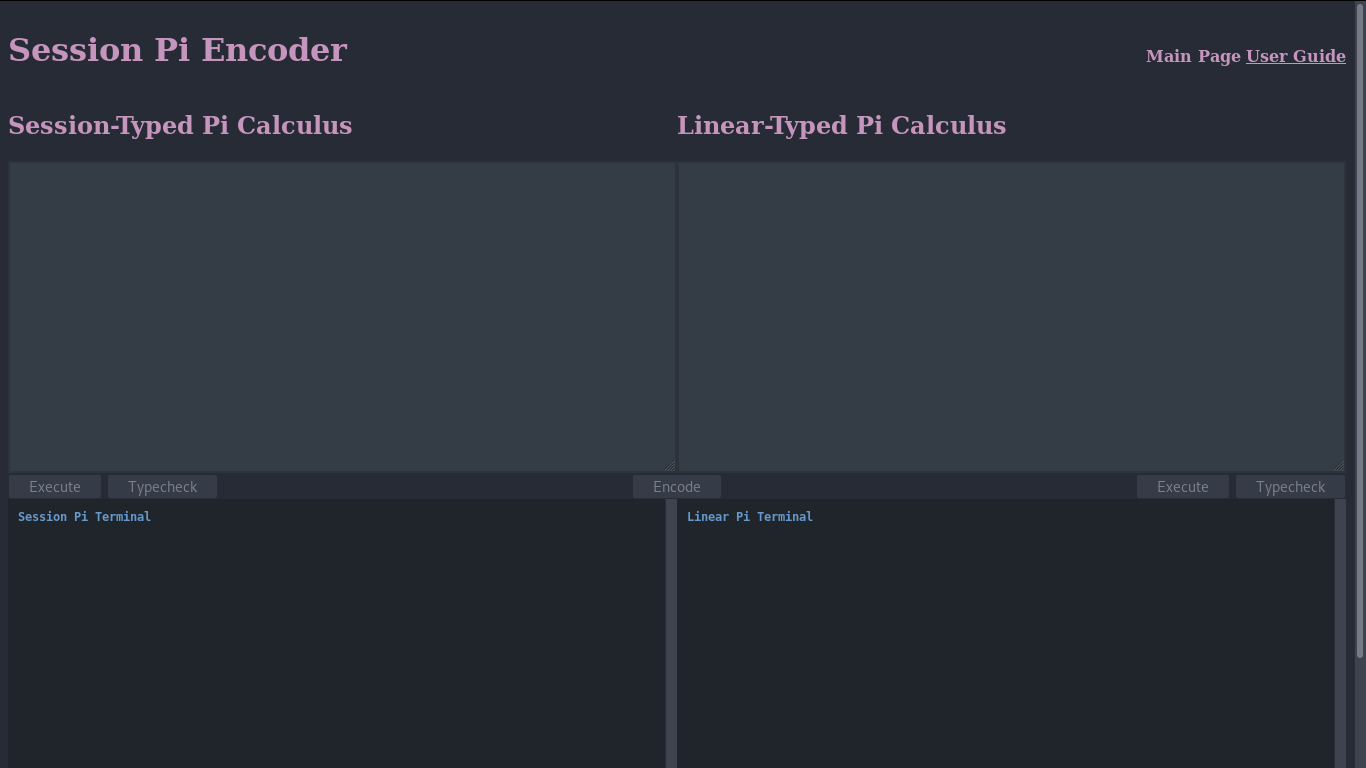
\includegraphics[width=\textwidth]{images/InterfaceScreenshotMain.png}
\caption{The web app's main page, as it appears when first accessing the web app. As described above, the top-left and top-right areas are input areas to type $\pi$-calculus code for session types and linear types respectively, and the bottom-left and bottom-right are the output areas for session types and linear types respectively. As there is no input in either of the input areas, the buttons are all disabled, and become enabled when there is text present in the appropriate input area.}
\label{fig:scshMain}
\end{figure}
\begin{figure}[H]
\centering
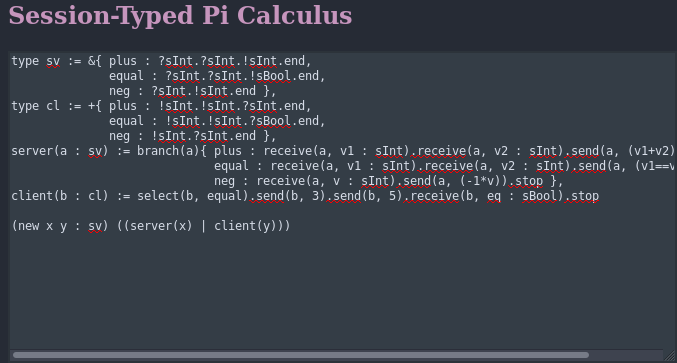
\includegraphics[width=\textwidth]{images/InterfaceScreenshotProcess.png}
\caption{The maths server example, entered into the session-typed $\pi$-calculus input area. The input areas have horizontal scrolling, as wrapping the text onto the next line was found to be difficult to read.}
\label{fig:scshProc}
\end{figure}

\quad The interface has 5 buttons that perform operations on the user's $\pi$-calculus code: An execute button for each of session-typed and linear-typed $\pi$-calculus, a typecheck button for each, and an encode button. The execute and encode buttons also typecheck the code alongside their own functionality. When code is typechecked, the interface produces a success message detailing the typing rules used. When code is executed, the interface displays a success message with a list of the reductions made as part of execution. Encoding from session-typed to linear-typed $\pi$-calculus produces a brief success message, and automatically inserts the encoded $\pi$-calculus into the input area for linear-typed $\pi$-calculus. Each of these can instead produce error messages, if some part of the operation is unsuccessful due to the user input containing incorrect or invalid $\pi$-calculus. Figures \ref{fig:scshSTCh}, \ref{fig:scshSSem}, \ref{fig:scshEnc}, \ref{fig:scshLTCh} and \ref{fig:scshLSem} show respectively the outputs of typechecking the maths server example in session types, executing it in session types, encoding it into linear types, typechecking the encoding, and executing the encoding.

\begin{figure}[H]
\centering
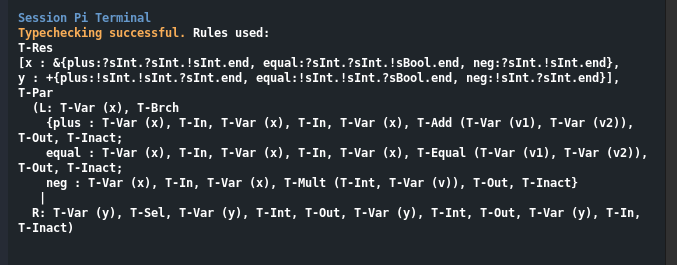
\includegraphics[width=\textwidth]{images/InterfaceScreenshotSTCh.png}
\caption{Typechecking in session-typed $\pi$-calculus. This is the typechecking output for the maths server example. T-Par structures the rest of the typing rules similarly to how the parallel composition structures its processes, to help readability of the output. Similarly, expressions contain the typing rules of their operands in parentheses after the typing rule for the expression itself. T-Res shows the types of the session endpoints it is restricting, and T-Var shows the name of the variable being checked.}
\label{fig:scshSTCh}
\end{figure}
\begin{figure}[H]
\centering
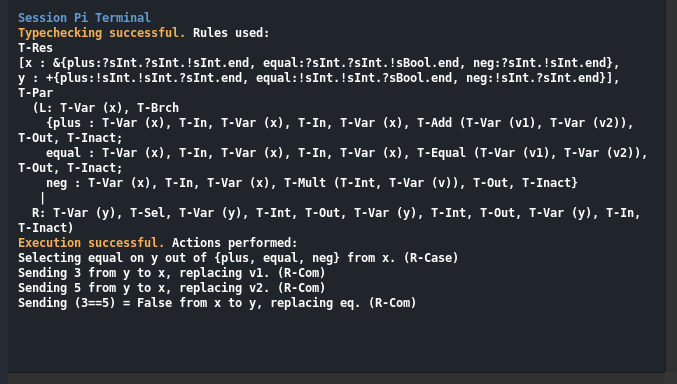
\includegraphics[width=\textwidth]{images/InterfaceScreenshotSesExe.png}
\caption{Execution of session-typed $\pi$-calculus. This is the execution output for the maths server example. Each message shows what message is being passed, and what bound variables are being replaced. Note also that the final message shows both the expression present in the output process and the value obtained from it that is the actual payload.}
\label{fig:scshSSem}
\end{figure}
\begin{figure}[H]
\centering
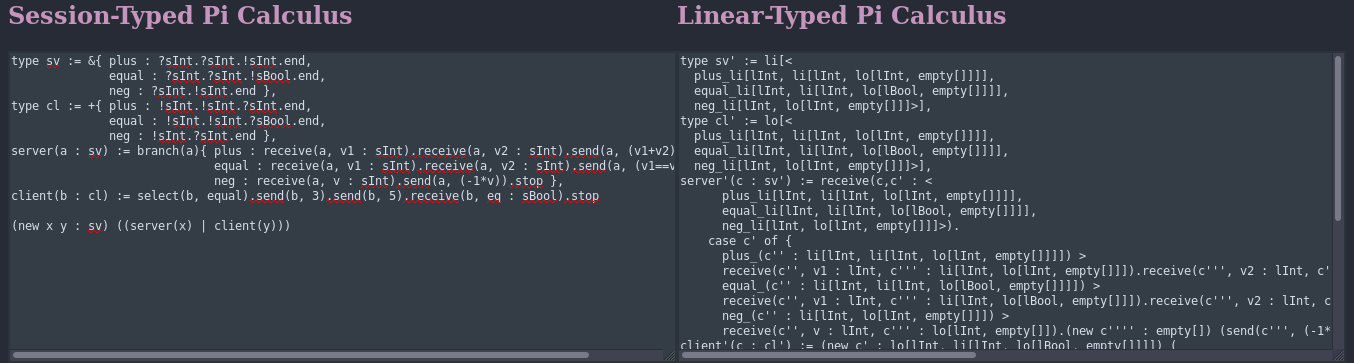
\includegraphics[width=\textwidth]{images/InterfaceScreenshotEnc.png}
\caption{Encoding from session-typed $\pi$-calculus into linear-typed $\pi$-calculus. This is the encoding of the maths server example. The encoded version is clearly much longer and more complicated, only part of it able to be shown in the input area at one time.}
\label{fig:scshEnc}
\end{figure}
\begin{figure}[H]
\centering
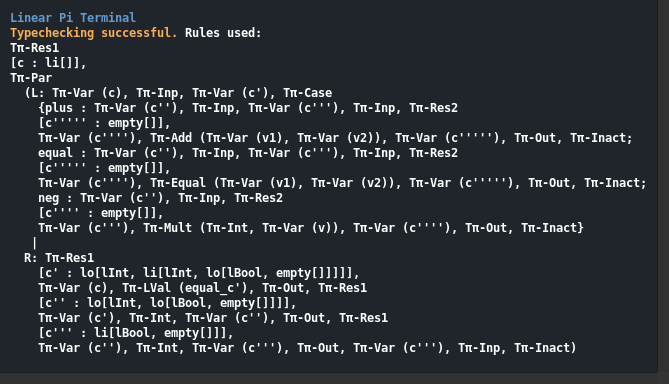
\includegraphics[width=\textwidth]{images/InterfaceScreenshotLinTCh.png}
\caption{Typechecking in linear-typed $\pi$-calculus. This is the typechecking output for the encoding of the maths server example. Much like the encoding itself, this is clearly much longer and more complicated than the typechecking output of the maths server example in session types. This is due to the inserted restrictions for continuation channels.}
\label{fig:scshLTCh}
\end{figure}
\begin{figure}[H]
\centering
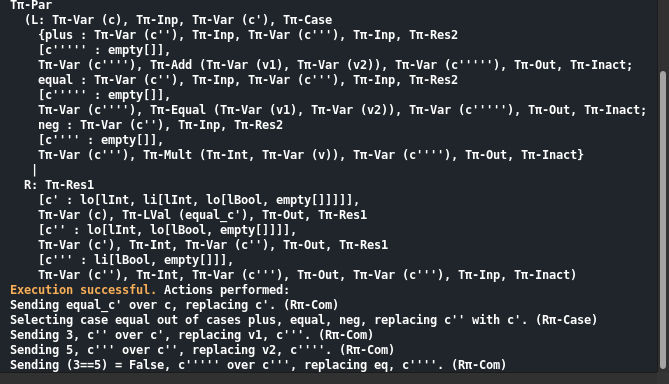
\includegraphics[width=\textwidth]{images/InterfaceScreenshotLinExe.png}
\caption{Execution of linear-typed $\pi$-calculus. This is the execution output for the encoding of the maths server example. Unlike the encoding itself and the typechecking output, semantics in linear types is not strongly complicated by the encoding, with only one extra reduction compared to the maths server example in session types.}
\label{fig:scshLSem}
\end{figure}

\quad As the web app is intended as a learning tool, it contains a user guide. The user guide details the syntax and explains the functionalities of $\pi$-calculus, to teach the user how to write valid and meaningful $\pi$-calculus code. It also contains sections detailing the typing rules, the encoding and the reduction rules used in execution, to give the user insight into how the web app performs these actions. There are also some minor notes on using the web app, such as things that produce unexpected results due to the parser being unable to interpret it as intended. Figure \ref{fig:scshGuide} shows the beginning of the user guide.

\begin{figure}[H]
\centering
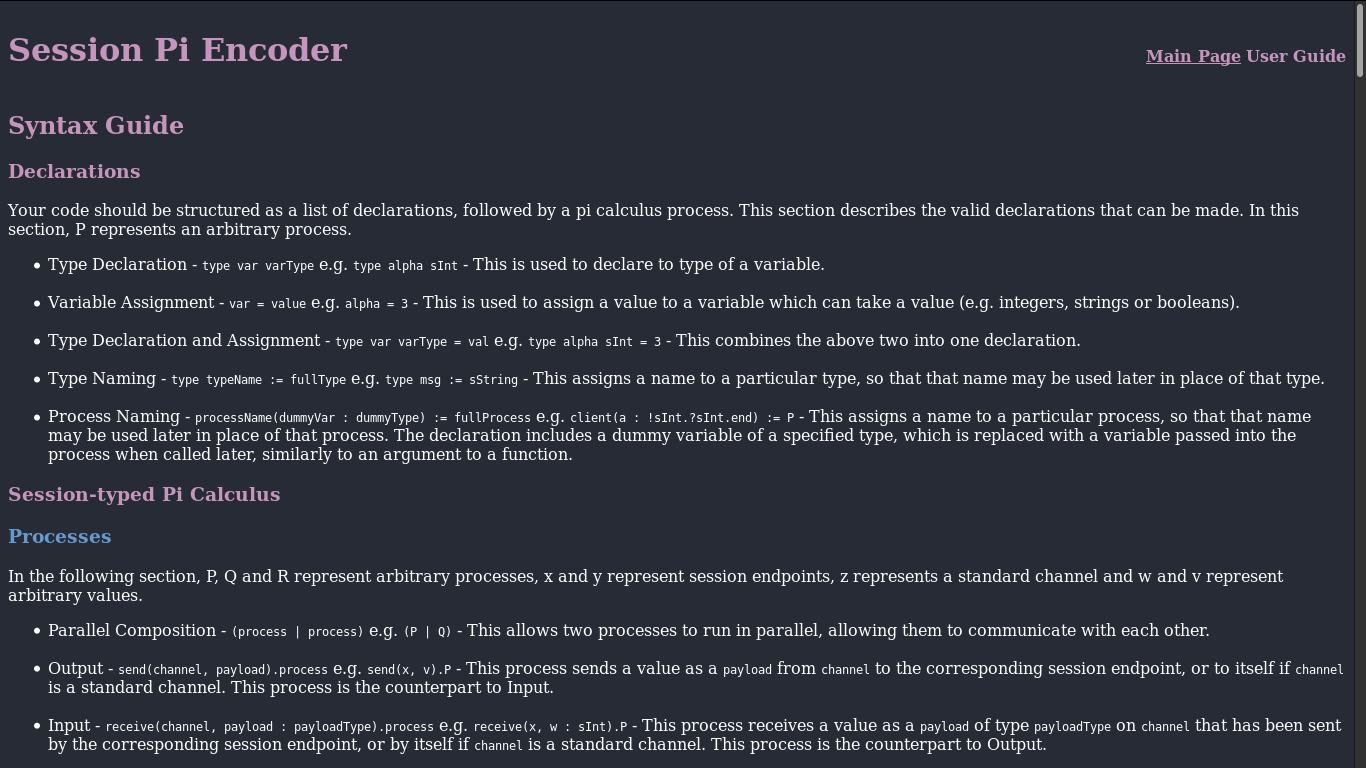
\includegraphics[width=\textwidth]{images/InterfaceScreenshotGuide.png}
\caption{The web app's user guide. The user guide begins with a syntax guide before explaining the concepts behind the actions of the web app, as the syntax is more important to being able to use the web app. The sections for typechecking, semantics and encoding use figures similar to those in this work.}
\label{fig:scshGuide}
\end{figure}

\quad The interface makes use of colour to draw attention to certain aspects of the app. In the main page, colours are used to draw attention to the labels of each section, making it clear what each section is, and are used in the output to give the user information on what has happened at a glance, e.g. when an action is performed successfully, the success message is highlighted in orange, while the details are plain, or if an error occurs, the error message is red. In the user guide, headers and sub-headers are coloured differently from each other to make the structure of the guide clear.


%==================================================================================================================================
\chapter{Implementation}
\label{implement}

\section{Architecture}
\label{implArch}

\quad The project is written in Python \citep{Python}, making use of Flask as a framework for the web app aspects of the project, and ANTLR for the language recognition aspects.

\quad Flask is a web development micro-framework written in Python. By micro-framework, the developers of Flask mean that "Flask aims to keep the core simple but extensible". \citep{FlaskDocs} Flask was chosen as the framework for the project for this reason. The web app is lightweight, not requiring any significant back-end technologies found in most web apps such as databases or user authentication. As many web app frameworks contain these features by default while Flask does not, Flask was an ideal candidate for the project.

\quad ANTLR, short for \textbf{AN}other \textbf{T}ool for \textbf{L}anguage \textbf{R}ecognition, is a parser generator. \citep{Antlr} Given a grammar for a language, ANTLR can automatically generate parsers that transform something written in that language into a syntax tree, and templates for programs that traverse that tree, performing some action at each node. This allows coders to easily create programming languages and other tools involving files fitting a custom-defined structure. ANTLR was chosen for the project as it allowed us to focus on the implementation of what should be done with the $\pi$-calculus code once it has been parsed, rather than the implementation of correctly parsing it.

\section{Web Interface}
\label{implInterface}

\quad The implementation of the web interface is primarily in the file \texttt{SPEncoder.py}. This file contains the code defining the Flask app, and connects the Flask app to the ANTLR code detailed in the following sections. It handles the main page and the user guide, which simply render HTML files \texttt{SPEncoder.html} and \texttt{SPEGuide.html} respectively.

\quad Whenever a button on the interface is pressed, the web app's JavaScript, defined in \texttt{SPEncoder.js}, gets the contents of the appropriate text area, and sends a request containing those contents to a certain URL, depending on which button is pressed. These URLs are connected to functions in \texttt{SPEncoder.py} that instantiate an ANTLR parser to which they give the code supplied by the JavaScript. They then instantiate the ANTLR listeners detailed in the following sections to perform the operation corresponding to the button pressed. The listeners produce an output, or an error message, and \texttt{SPEncoder.py} returns them as JSON to \texttt{SPEncoder.js}, which inserts them into the appropriate elements. This is coded using AJAX, so that the results appear dynamically.

\section{Encoding}
\label{implEncode}

\quad The encoding is implemented as part of an ANTLR listener, \texttt{SPEListener.py}. This listener also contains the code to perform the typechecking, as detailed in Section \ref{implTCh}, which it can do concurrently with the encoding. For a program in session-typed $\pi$-calculus code, the encoding of this program is generated by constructing a string of the encoding from information in each of the nodes of the syntax tree.

\quad Before the encoding begins, a separate listener \texttt{VariableNameCollector.py} is run to form a list of variable names the user has used in their code. This is done to ensure that none of the new channels generated by the encoding use a pre-existing name. Generated channels only use names of the form \texttt{c}, \texttt{c'}, \texttt{c''}, etc. which users are advised in the user guide not to use, but \texttt{VariableNameCollector.py} is used in case users don't follow this advice.

\quad The encoding starts as a string containing a placeholder, to be used as a string builder. Each rule of the grammar has corresponding functions which replace the first placeholder in the string builder with a string representing the encoding of that rule, the string typically containing more placeholders itself. Different placeholders are used to represent processes, types, declarations, etc. A dictionary is used to act as the encoding function. 

\quad As the encoding inserts new restrictions and new payloads, these restrictions and the input processes containing these payloads need additional type annotations. These were generated using a dictionary \texttt{contChanTypes} to keep track of the type of session endpoints at the current point in the process. When an inserted type annotation needs to be generated, a new parse tree walker is created to traverse the current saved type of the session endpoint, using the current listener instance. This essentially temporarily redirects the tree traversal of the listener to the session endpoint's type, after which it returns to where it was in the process.

\quad Stacks are used in the listener for multiple purposes, such as to keep old copies of the encoding function, and replace the current encoding function with these copies when appropriate. For example, when encoding a branch process with two branches \texttt{alpha} and \texttt{beta}, a copy of the encoding function is saved to a stack, and then the process \texttt{alpha} is encoded. After this, the encoding function is replaced with the saved copy from before \texttt{alpha} was encoded, and the process \texttt{beta} is encoded with this copy, so that the encoding of \texttt{beta} does not use variables created in \texttt{alpha}.

\quad Listing \ref{lst:encCode} presents as an example the function \texttt{enterInputSesEnc}, used to encode a session-typed output process.

\begin{lstlisting}[language=Python, float=p, caption={\texttt{enterInputSesEnc}, the function used to encode a session-typed input process. \texttt{ctx} is the ANTLR context of the current instance of the grammar rule. It is the object containing everthing found within this instance, such as the ANLTR contexts of instances of other grammar rules that appear within this instance's rule. \texttt{self.checkBranchStack} and \texttt{self.checkCompStack} check whether the current process is the initial process in the continuation of a branch or an arm of a parallel composition respectively and the encoding function or list of existing variable names should therefore be reset. These functions are both passed a parameter \texttt{False} to indicate the current process is not a branch or composition respectively. The \texttt{if} statement checks if the input process uses a standard channel, and gives a simpler encoding if so. The {else} clause generates a new channel name, updates \texttt{contChanTypes}, adds the payload to \texttt{contChanTypes} if it is a channel, adds the new channel to the encoding function and adds the encoded string to the string builder. It then encodes the type of the newly generated type annotation. $\CIRCLE$ is used as a placeholder for processes, $\blacktriangle$ is used as a placeholder for types and $\star$ is used so that type annotations are inserted in the correct order.}, label={lst:encCode}, extendedchars=True, numbers=left]
def enterInputSesEnc(self, ctx):
	self.checkBranchStack(False)
	self.checkCompStack(False)
	if isinstance(self.contChanTypes[ctx.channel.getText()], PiCalcParser.ChannelTypeContext):
		self.encodedStrBuilder = self.encodedStrBuilder.replace(u"(*@$\CIRCLE$@*)", "receive(" + ctx.channel.getText() + ", " + ctx.payload.getText() + u" : (*@$\blacktriangle$@*)).(*@$\CIRCLE$@*)", 1)
	else:
		ipStrBuilder = "receive(" + self.encodeName(ctx.channel.getText()) + ", " + ctx.payload.getText() + u" : (*@$\star$@*)"
		newChan = self.generateChannelName()
		newChanType = self.contChanTypes[ctx.channel.getText()].sType()
		self.contChanTypes[ctx.channel.getText()] = newChanType
		if isinstance(ctx.plType, PiCalcParser.SessionTypeContext):
			self.contChanTypes[ctx.payload.getText()] = ctx.plType.sType()
		elif isinstance(ctx.plType, PiCalcParser.ChannelTypeContext):
			self.contChanTypes[ctx.payload.getText()] = ctx.plType
		ipStrBuilder = ipStrBuilder + ", " + newChan + u" : (*@$\blacktriangle$@*)).(*@$\CIRCLE$@*)"
		self.encFunc[ctx.channel.getText()] = newChan
		self.encodedStrBuilder = self.encodedStrBuilder.replace(u"(*@\CIRCLE@*)", ipStrBuilder, 1)
		typeWalker = ParseTreeWalker()
		typeWalker.walk(self, newChanType)
		self.encodedStrBuilder = self.encodedStrBuilder.replace(u"(*@$\star$@*)", u"(*@$\blacktriangle$@*)", 1)
\end{lstlisting}

\newpage

\section{Typechecking}
\label{implTCh}

\quad Typechecking is implemented in \texttt{SPEListener.py}. Given a program in either session- or linear-typed $\pi$-calculus, the listener traverses the syntax tree of this program, applying typing rules as appropriate and generating an output string detailing what typing rules it applies.

\quad The listener starts by collecting types from the type declarations at the start of the program, if there are any. Once it has looked at all of these, it now has the initial typing context \texttt{gamma}. It then begins traversing the processes. As many of the process typing rules involve the context split or context combination operator and using one of the separated typing contexts in another typing rule, the listener needs some way of saving contexts for later, which is accomplished through the \texttt{gammaStack}. For all typing rules, the current typing context is retrieved from the stack, premises of the typing rule which do not involve another typing rule are checked, and then any typing contexts that are used to check another typing rule in the premise are added to the stack so that those can be checked when the listener's traversal reaches them.

\quad \texttt{VariableNameCollector.py} is also used in the typechecking, this time to aid the context split or context combination operators. When using these operators, a list of variable names is used to decide which linear types should go into which of the separated typing contexts, those in the list going into the first, all others into the second. In T-Par and T$\pi$-Par, \texttt{VariableNameCollector.py} is used to collect all of the variable names used in the left arm of the parallel composition, so that these are placed into the first typing context. For T$\pi$-Par, \texttt{VariableNameCollector.py} can also collect what each channel is used for, i.e. which capability of a linear channel appears in the left arm of the parallel composition.

\quad Listing \ref{lst:sTChCode} presents as an example the function \texttt{enterInputSesSTCh}, the function used to typecheck a session-typed input process. The function \texttt{enterInputLinLTCh}, used to typecheck a linear-typed input process, is presented in Listing \ref{lst:lTChCode}. Note the names of these functions, \texttt{InputSesSTCh} and \texttt{InputLinLTCh}, each contain two references to which typing system is used. This is because the naming convention we used for typechecking in session types is to add \texttt{STCh} to the function name, and \texttt{LTCh} for linear types, for example \texttt{enterOutputSTCh} and \texttt{enterOutputLTCh}. However, input processes are defined with two separate grammar rules \texttt{InputSes} and \texttt{InputLin}, so that an input process's type annotations may contain either session types or linear types. The functions \texttt{enterInputSesLTCh} and \texttt{enterInputLinSTCh} do exist, but as they are not meaningful, they simply throw errors and cause the typechecking to fail.

\begin{lstlisting}[language=Python, float=p, caption={\texttt{enterInputSesSTCh}, the function used to typecheck a session-typed input process. \texttt{ctx} is as described in Listing \ref{lst:encCode}. \texttt{self.getReplacement} returns the variable which replaces the channel or payload, should either of those be the dummy variable of a process naming declaration. \texttt{self.splitGamma} represents the context split operator. It is passed the typing context to split and a list of variables which if linear should be placed in the first context, with all other linear variables placed in the second. The function then retrieves the types of the channel and the payload, and checks if the channel is a standard channel or a receive session. It then checks that the type of the payload matches the channel type's payload type. The function then prepares the typing context for the continuation process and adds the typing rule into the typechecking output. \texttt{self.printVariableTypeRule} inserts into the typechecking output the typing rule for the channel i.e. T-Var. The final \texttt{else} clause is the code for rule T-StndIn and is near identical to lines 16-29, so it has been omitted for sake of brevity. $\square$ is used as a placeholder for typing rules, $\triangle$ is used as a placeholder for commas as a separator between the rules.}, label={lst:sTChCode}, extendedchars=True, numbers=left]
def enterInputSesSTCh(self, ctx):
	self.gamma = self.gammaStack.pop()
	trueChan = self.getReplacement(ctx.channel)
	truePL = self.getReplacement(ctx.payload)
	(gamma1, gamma2) = self.splitGamma(self.gamma, [trueChan.getText()])
	chanType = gamma1.get(trueChan.getText())
	payloadType = ctx.tType()
	if isinstance(payloadType, PiCalcParser.BasicSesTypeContext):
		payloadType = payloadType.basicSType()
	elif isinstance(payloadType, PiCalcParser.SessionTypeContext):
		payloadType = payloadType.sType()
	if not isinstance(chanType, PiCalcParser.ChannelTypeContext):
		if not isinstance(chanType, PiCalcParser.ReceiveContext):
			self.tcErrorStrBuilder = self.tcErrorStrBuilder = "<span class='error'>ERROR: Typechecking rule T-In failed due to " + trueChan.getText() + ". Input process on channel not of receive type.</span>\n"
			raise self.typecheckException
		chanPLType = chanType.tType()
		if isinstance(chanPLType, PiCalcParser.BasicSesTypeContext):
			chanPLType = chanPLType.basicSType()
		elif isinstance(chanPLType, PiCalcParser.SessionTypeContext):
			chanPLType = chanPLType.sType()
		if not isinstance(payloadType, type(chanPLType)):
			self.tcErrorStrBuilder = self.tcErrorStrBuilder = "<span class='error'>ERROR: Typechecking rule T-In failed due to " + truePL.getText() + ". Input process payload has type annotation that does not match channel type.</span>\n"
			raise self.typecheckException
		else:
			augmentations = {trueChan.getText(): chanType.sType(), truePL.getText(): chanPLType}
			gamma2 = self.augmentGamma(gamma2, augmentations)
			self.gammaStack.append(gamma2)
			self.typeCheckStrBuilder = self.typeCheckStrBuilder.replace(u"(*@$\square$@*)", u"(*@$\square\triangle$@*)T-In(*@$\triangle\square$@*)", 1)
			self.printVariableTypeRule(trueChan, gamma1)
	else: (...)
\end{lstlisting}

\begin{lstlisting}[language=Python, float=p, caption={\texttt{enterInputLinLTCh}, the function used to typecheck a linear-typed input process. This function works similiarly to \texttt{enterInputSesSTCh}, detailed in Listing \ref{lst:sTChCode}. The main differences are the use of \texttt{self.combineGamma} instead of \texttt{self.splitGamma} and the handling of multiple payloads. The final \texttt{else} clause has again been omitted for brevity and similarity to lines 16-29.}, label={lst:lTChCode}, extendedchars=True, numbers=left]
def enterInputLinLTCh(self, ctx):
	self.gamma = self.gammaStack.pop()
	trueChan = self.getReplacement(ctx.channel)
	truePLs = [self.getReplacement(pl) for pl in ctx.payloads]
	(gamma1, gamma2) = self.combineGamma(self.gamma, [(trueChan.getText(), "Input")])
	chanType = gamma1.get(trueChan.getText())
	payloadTypes = copy.deepcopy(ctx.plTypes)
	for i in range(len(payloadTypes)):
		if isinstance(payloadTypes[i], PiCalcParser.BasicLinTypeContext):
			payloadTypes[i] = payloadTypes[i].basicLType()
	if not isinstance(chanType, PiCalcParser.ConnectionContext):
		if not isinstance(chanType, PiCalcParser.LinearInputContext):
			self.tcErrorStrBuilder = self.tcErrorStrBuilder + "<span class='error'>ERROR: Typechecking rule T(*@$\pi$@*)-Inp failed due to " + trueChan.getText() + ". Input process on channel not of input type.</span>\n"
			raise self.typecheckException
		else:
			augmentations = {}
			chanPLTypes = chanType.payloads
			for i in range(len(payloadTypes)):
				if isinstance(chanPLTypes[i], PiCalcParser.BasicLinTypeContext):
					chanPLTypes[i] = chanPLTypes[i].basicLType()
				if not isinstance(payloadTypes[i], type(chanPLTypes[i])):
					self.tcErrorStrBuilder = self.tcErrorStrBuilder + "<span class='error'>ERROR: Typechecking rule T(*@$\pi$@*)-Inp failed due to " + truePLs[i].getText() + ". Input process payload has type annotation that does not match channel type.</span>\n"
					raise self.typecheckException
				augmentations[truePLs[i].getText()] = chanPLTypes[i]
			gamma2 = self.augmentGamma(gamma2, augmentations)
			self.gammaStack.append(gamma2)
			self.typeCheckStrBuilder = self.typeCheckStrBuilder.replace(u"(*@$\square$@*)", u"(*@$\square\triangle$@*)T(*@$\pi$@*)-Inp(*@$\triangle\square$@*)", 1)
			self.printVariableTypeRule(trueChan, gamma1)
	else: (...)
\end{lstlisting}

\newpage

\section{Semantics}
\label{implSem}

\quad Operational semantics of $\pi$-calculus are implemented in an ANTLR listener \texttt{SPERunner.py}. Given a program in session- or linear-typed $\pi$-calculus code, it executes the program by repeatedly checking for reductions between pairs of processes and applying them, until no more reductions can be made. For each reduction it makes, it records for the output what this reduction does.

\quad The listener starts by parsing the declarations, gathering any variables to which values are assigned, then parsing the process, collecting information on what channels exist and what they communicate with from restrictions. Once the parser reaches a parallel composition, it creates a list containing the composed processes. This list begins simply as the two arms of the initial parallel composition, but the listener then refines the list by checking if these are restrictions or nested compositions, and gathering processes from these. Once the final list of composed processes has been found, where all of the processes are some process on which a reduction can occur, the listener starts checking for pairs of processes which can be reduced. 

\quad When it has found such a pair, e.g. an output process and an input process, it checks the channels to see if these processes are communicating. If they are, it then performs the reduction, replacing the processes in the list with their continuations, and saving what bound variables have been replaced as a result of communication. After all pairs have been checked, the listener checks whether all processes are terminated. The listener will then finish execution successfully, begin a new cycle of checking for reductions, or finish execution unsuccessfully, depending on whether all processes are terminated, not all processes are terminated and a reduction was made this cycle, or not all processes are terminated and no reduction was made this cycle.

Listing \ref{lst:sReducCode} presents as an example the implementation of the reduction rules R-Com and R-StndCom.

\begin{lstlisting}[language=Python, float=p, caption={The implementation of the reduction rules R-Com and R-StndCom. \texttt{self.parProcs} is the list of processes composed in parallel, and \texttt{self.chanCounterparts} is a list recording where each channel communicates with, i.e. itself if it is a standard or linear channel, or its co-name if it is a session endpoint. \texttt{self.getReplacement} returns what a variable has been replaced by as a result of communication, if it has been replaced. Once the listener has determined that the processes can communicate, it checks if the payload is an expression, and evaluates it if so, and if not, it checks if it is a named variable with an assigned value. In either of these cases, the value of the payload is printed in the output along with the payload itself. The input process's payload variable is replaced with the output process's. The listener then checks if the reduction rule being applied is R-Com or R-StndCom, and adds the appropriate string to the execution output. The list of processes composed in parallel is updated with the continuation processes, and the listener makes a note that a successful reduction was made.}, label={lst:sReducCode}, extendedchars=True, numbers=left]
if isinstance(self.parProcs[i], PiCalcParser.OutputContext) and isinstance(self.parProcs[j], PiCalcParser.InputSesContext):
	if (self.getReplacement(i, self.parProcs[i].channel).getText() == self.chanCounterparts[self.getReplacement(j, self.parProcs[j].channel).getText()]) and (self.getReplacement(j, self.parProcs[j].channel).getText() == self.chanCounterparts[self.getReplacement(i, self.parProcs[i].channel).getText()]):
		payloadText = self.getReplacement(i, self.parProcs[i].payloads[0]).getText()
		if isinstance(self.parProcs[i].payloads[0], PiCalcParser.ExprValueContext):
			evalExpr = self.evaluateExpression(self.parProcs[i].payloads[0].expression(), i)
			payloadText = self.printExpression(self.parProcs[i].payloads[0].expression(), i) + " = " + evalExpr.getText()
			self.replacements[j][self.parProcs[j].payload.getText()] = evalExpr
		else:
			if isinstance(self.getReplacement(i, self.parProcs[i].payloads[0]), PiCalcParser.NamedValueContext) and self.getReplacement(i, self.parProcs[i].payloads[0]).getText() in self.variableValues:
				payloadText = payloadText + " = "  + self.variableValues[self.getReplacement(i, self.parProcs[i].payloads[0]).getText()].getText()
			self.replacements[j][self.parProcs[j].payload.getText()] = self.getReplacement(i, self.parProcs[i].payloads[0])
		if self.getReplacement(i, self.parProcs[i].channel).getText() == self.getReplacement(j, self.parProcs[j].channel).getText():
			self.executionStrBuilder = self.executionStrBuilder + "Sending " + payloadText + " over " + self.getReplacement(i, self.parProcs[i].channel).getText() + ", replacing " + self.parProcs[j].payload.getText() + ". (R-StndCom)\n"
		else:
			self.executionStrBuilder = self.executionStrBuilder + "Sending " + payloadText + " from " + self.getReplacement(i, self.parProcs[i].channel).getText() + " to " + self.getReplacement(j, self.parProcs[j].channel).getText() + ", replacing " + self.parProcs[j].payload.getText() + ". (R-Com)\n"
		self.parProcs[i] = self.parProcs[i].processSec()
		self.parProcs[j] = self.parProcs[j].processSec()
		reductionMade = True
\end{lstlisting}

%==================================================================================================================================
\chapter{Evaluation} 
\label{evaluation}

\section{User Study}
\label{evalStudy}

\quad To evaluate how effective the web app is as a teaching tool, we performed a user study. We gave participants access to the web app, and a survey asking them to perform some tasks in the web app and then rate their experience. The full survey can be seen in Appendix \ref{appSurvey}. Participants were gathered in the following way:
\begin{itemize}
    \item One group of 5 participants who were not already familiar with $\pi$-calculus.
    \item One group of 5 participants who had been formally taught $\pi$-calculus, in the Theory of Computation course. Of this group:
    \begin{itemize}
        \item 3 participants had taken Theory of Computation in the academic year 2017-2018, and so had not been formally taught session types.
        \item 2 participants had taken Theory of Computation in the academic year 2018-2019, and so had been formally taught session types.
    \end{itemize}
\end{itemize}

\quad Participants already familiar with $\pi$-calculus were used to make sure that the web app was not attempting to teach $\pi$-calculus in a way so different from how it is normally taught that it would confuse anyone who had previously learned it in those ways, and so it would still be usable by people already familiar.

\quad The main aims of the user study were the following:
\begin{description}
    \item [Aim 1] Find out how well participants felt the user guide explains the concepts of typechecking, semantics and the encoding
    \item [Aim 2] Find out how well participants felt the user guide had taught them about writing $\pi$-calculus code.
    \item [Aim 3] Find out how the participants felt the web app had affected their understanding of session types and linear types
    \item [Aim 4] Find out how the participants felt the web app had affected their understanding of $\pi$-calculus.
    \item [Aim 5] Find out how the modified syntax might affect the usability of the site for those already experience with $\pi$-calculus.
\end{description}

\quad The survey in the user study started by asking participants how familiar they already were with $\pi$-calculus and with session types and linear types. This was done so that the results could be considered in the same groups that participants were gathered in, as although we knew beforehand which group each participant was in, the results are stored anonymously. Charts of the responses to these introductory questions can be seen in Figure \ref{fig:fmlrPiCalc} and Figure \ref{fig:fmlrSesLin}.

\begin{figure}[H]
\centering
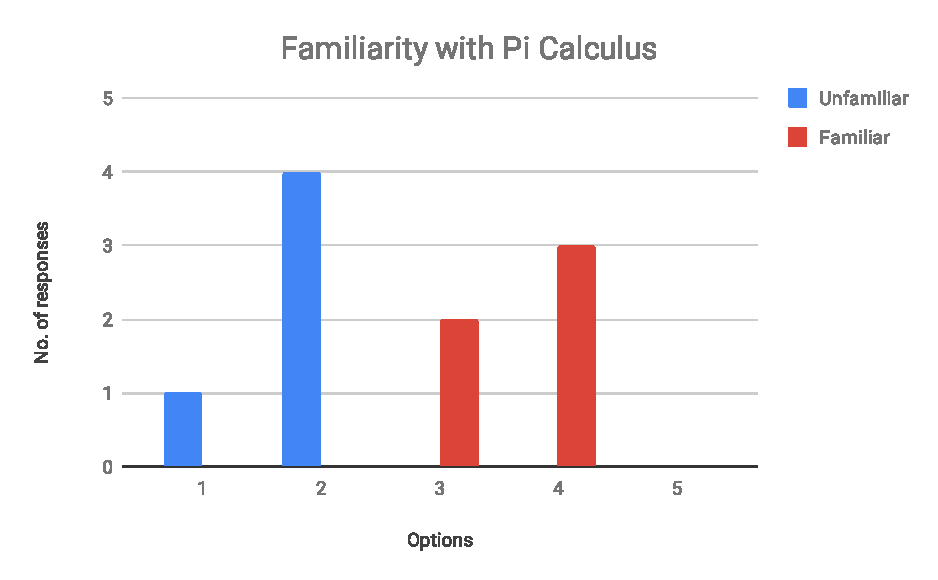
\includegraphics[width=0.72\textwidth]{images/PiCalcFamiliar.pdf}
\caption{The responses to the question asking how familiar participants are with $\pi$-calculus. Options ranged from 1 to 5, 1 being labelled "Never heard of $\pi$-calculus" and 5 being labelled "Very familiar with $\pi$-calculus". As expected, all participants from the group not already familiar with $\pi$-calculus answered lower than all participants from the group already familiar.}
\label{fig:fmlrPiCalc}
\end{figure}

\begin{figure}[H]
\centering
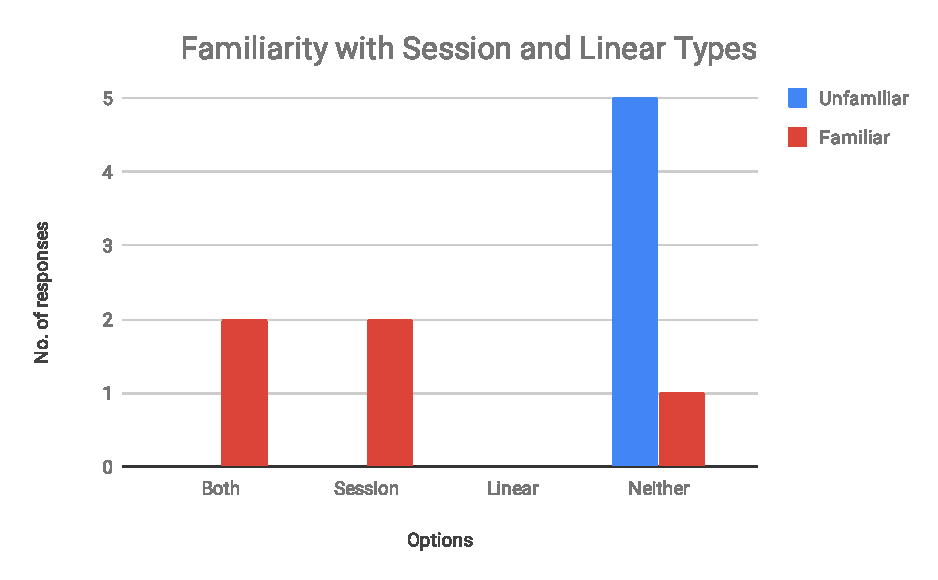
\includegraphics[width=0.72\textwidth]{images/SesLinFamiliar.pdf}
\caption{The responses to the question asking how familiar participants are with session types and linear types in $\pi$-calculus. As expected, no participants in the group unfamiliar with $\pi$-calculus were familiar with session types or linear types in $\pi$-calculus. Those already familiar with $\pi$-calculus were a mixture of people familiar and unfamiliar with session types or linear types.}
\label{fig:fmlrSesLin}
\end{figure}

\quad The survey then prompted the participants to read the web app's user guide, and then perform three tasks in the web app. The survey did not record any information directly related to the participant's performance in these tasks. The first of these tasks was to examine an example program and consider how this program would typecheck, execute and encode, then to perform all three of these actions in the web app and compare the results to what they expected. This was designed to achieve \textbf{Aim 1}. 

\quad The second task gave them an incomplete example program containing a \texttt{branch} process with three branches, and asked the participants to write processes which would act as the counterpart to each branch. This was designed to achieve \textbf{Aim 2}. 

\quad The third task gave an example program which did not work and would throw errors when typechecked, and asked users to identify why. It then asked them to correct the issue with the program, so that it can successfully be typechecked, executed and encoded. This task was also designed to achieve \textbf{Aim 2}, but by checking their understanding of what is not valid $\pi$-calculus, rather than what is.

\quad To gather the participants opinions on the web app, once they had finished all tasks, the survey asked them questions on how easy or difficult they found it to understand the user guide, understand the example programs, write $\pi$-calculus code and correct $\pi$-calculus code. It then also asked them how they felt the user study had affected their understanding of session types and linear types, and of $\pi$-calculus, to achieve \textbf{Aims 3 and 4}. Charts of the responses to these questions can be seen in Figures \ref{fig:UndStndGuide}, \ref{fig:UndStndExamples}, \ref{fig:WriteCode}, \ref{fig:CorrectCode}, \ref{fig:PiCalcImprov} and \ref{fig:SesLinImprov}. 

\begin{figure}[H]
\centering
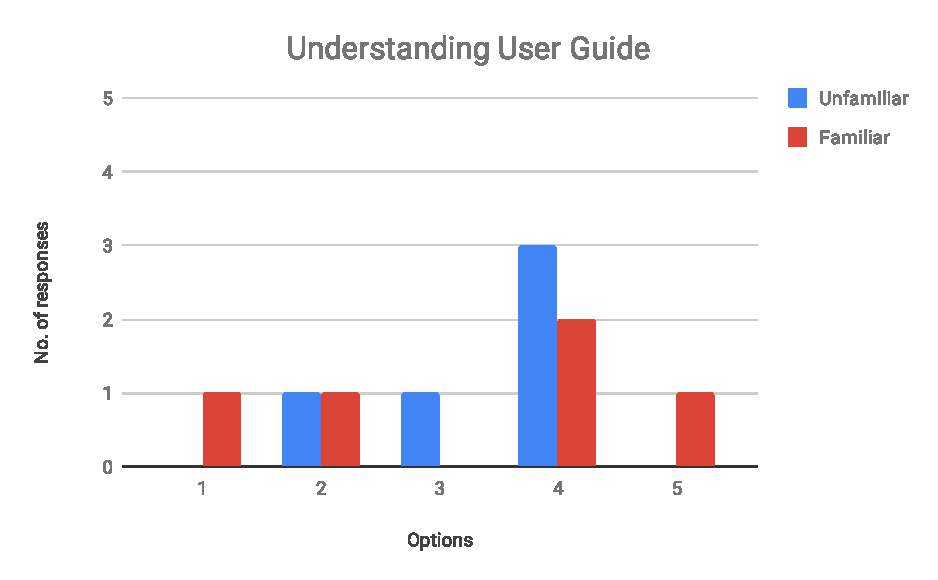
\includegraphics[width=0.72\textwidth]{images/UndStndGuide.pdf}
\caption{Responses to the question asking how easy or difficult participants found it to understand the web app's user guide. Options ranged from 1 to 5, 1 being "Very difficult", 5 being "Very easy". Results are mixed, leaning towards the user guide being easy to understand, showing that it is generally helpful but could use improvement.}
\label{fig:UndStndGuide}
\end{figure}

\begin{figure}[H]
\centering
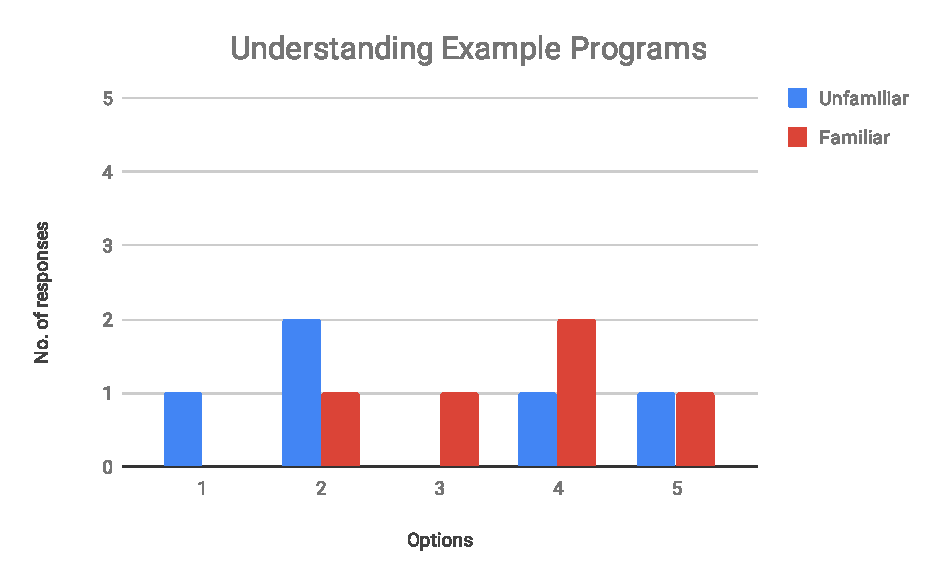
\includegraphics[width=0.72\textwidth]{images/UndStndExamples.pdf}
\caption{Responses to the question asking how easy or difficult participants found it to understand the examples programs from the survey. Options ranged from 1 to 5, 1 being "Very difficult", 5 being "Very easy". Results are mixed, showing that the syntax guide may not be sufficiently clear.}
\label{fig:UndStndExamples}
\end{figure}

\begin{figure}[H]
\centering
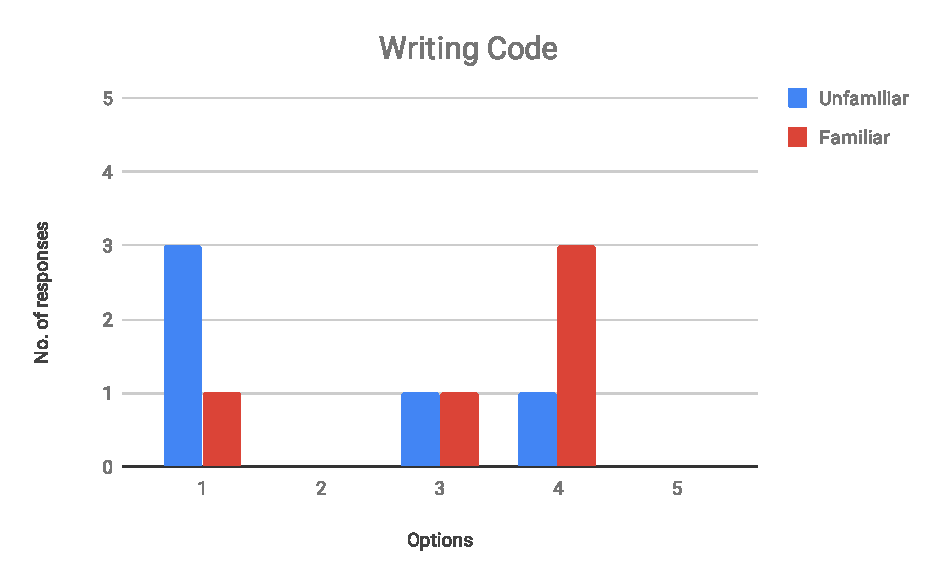
\includegraphics[width=0.72\textwidth]{images/WriteCode.pdf}
\caption{Responses to the question asking how easy or difficult participants found it to write their own $\pi$-calculus code. Options ranged from 1 to 5, 1 being "Very difficult", 5 being "Very easy". Many participants not already familiar with $\pi$-calculus struggled with this, showing that the user guide may not explain coding sufficiently well.}
\label{fig:WriteCode}
\end{figure}

\begin{figure}[H]
\centering
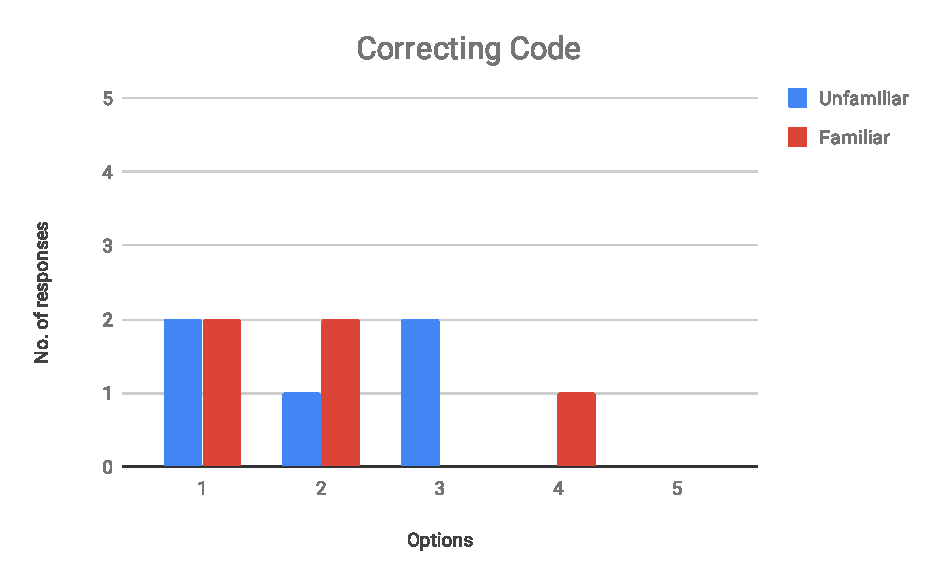
\includegraphics[width=0.72\textwidth]{images/CorrectCode.pdf}
\caption{Responses to the question asking how easy or difficult participants found it to correct faulty $\pi$-calculus code. Options ranged from 1 to 5, 1 being "Very difficult", 5 being "Very easy". Results are largely negative. However, we think this may be due to the specific example used, as the flaw in the code was a channel restriction only encompassing two out of the three composed processes. This flaw is identified by the placement of parentheses, and so is not easily noticable. This example therefore may not have been the most suitable, and had an example with a less subtle flaw been used, the results of this question may have been different.}
\label{fig:CorrectCode}
\end{figure}

\begin{figure}[H]
\centering
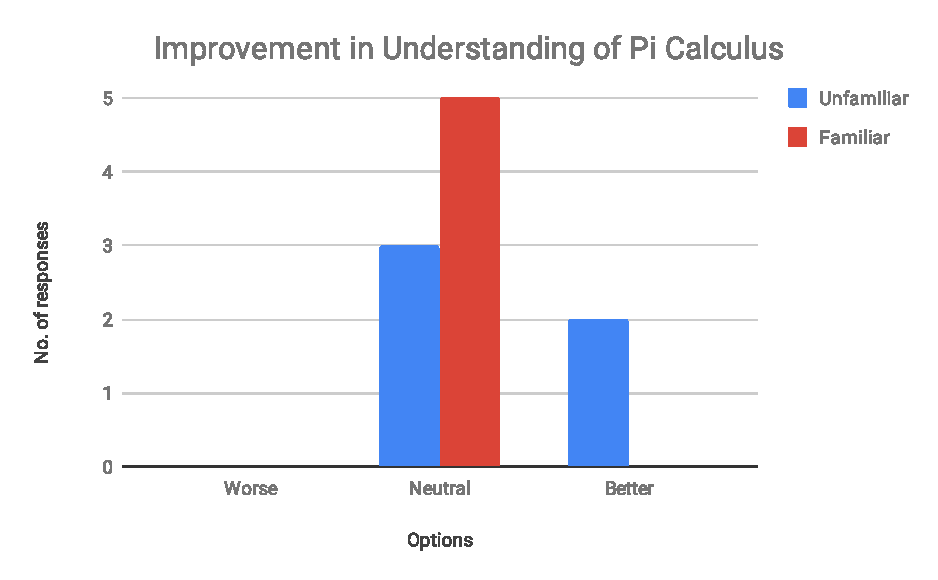
\includegraphics[width=0.72\textwidth]{images/PiCalcImprov.pdf}
\caption{Responses to the question asking how the web app has affected the participant's understanding of $\pi$-calculus. As expected, those already familiar did not feel they had learned anything new. Some of those unfamiliar did feel they had learned about $\pi$-calculus, but more did not feel any more knowledgeable, showing that the web app may not be as effective as a teaching tool as hoped.}
\label{fig:PiCalcImprov}
\end{figure}

\begin{figure}[H]
\centering
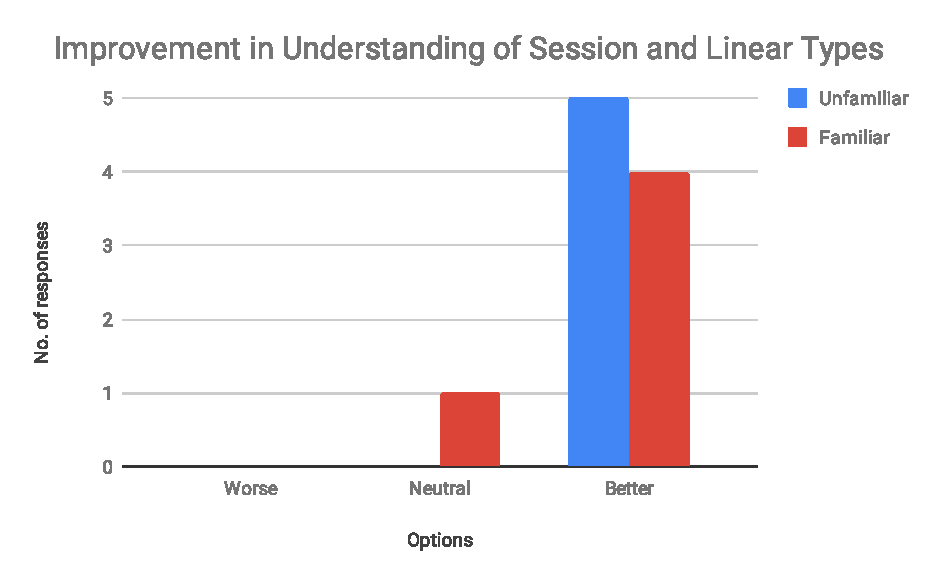
\includegraphics[width=0.72\textwidth]{images/SesLinImprov.pdf}
\caption{Responses to the quesiton asking how the web app has affected the participant's understanding of session types and linear types. Almost all participants felt their understanding had been improved, showing that the web app is effective in teaching the concepts of session and linear types.}
\label{fig:SesLinImprov}
\end{figure}

\quad Participants already familiar with $\pi$-calculus were also asked for comments on the web app's syntax, in comparison to the standard syntax. The responses are as follows:
\begin{itemize}
    \item "I personally prefer the standard syntax, as it's easier for me to read matching communications"
    \item "Both standard picalc syntax and the syntax of the webapp's picalc are VERY difficult to read due to how visually dense they are, plus how horizontal they are. I found myself constantly having to scroll horizontally to read various parts of the code, which hindered my understanding."
    \item "Seems a little bit more annoying to write with"
    \item 2 participants did not give any comment.
\end{itemize}
\quad This question was used to achieve \textbf{Aim 5}. As can be seen, the web app's syntax was not preferable to the standard syntax among those who chose to comment. \textbf{This result is unsurprising, as the syntax modification was made with new users in mind}.

\quad Overall, the results show that \textbf{while the web app succeeded in teaching most participants about session types and linear types, it was less successful in teaching them about $\pi$-calculus itself}. Additionally, while the user guide was generally helpful, there is room for improvement. As most of the troubles participants had appears to be with code, these improvements would likely come in the form of more detailed explanations of the processes, and perhaps including an example program in the user guide to help illustrate how the code is to be formed.

\quad In hindsight, while the user study did give valuable information on the effectiveness of the web app as a teaching tool, more information could've been gathered with better questions. For example, while participants with experience of $\pi$-calculus were asked for comments on the syntax, inexperienced participants were not. Asking these users about the syntax could have been a valuable way of finding out whether the web app's syntax is in fact easier to understand, as is hoped. Additionally, some participants commented on the lack of a question asking for general comments about the web app. This could have given us an idea of why, for example, they found the user guide difficult to understand, and thus how it can be improved to be more helpful.

\quad As none of the participants had been formally taught of the encoding, there was little focus on this in the user study, being mentioned only in the first task. In hindsight, this is perhaps something that should have been more prominent in the evaluation, as it is a major focus of the overall project.

\quad A signed ethics checklist, denoting that the user study complied with the ethics requirements of the University of Glasgow's School of Computing Science, can be found in Appendix \ref{appEthics}. The introduction and debriefing scripts used in the user study can be found in Appendices \ref{appIntro} and \ref{appDebrief} respectively.


%==================================================================================================================================
\chapter{Conclusion}
\label{conclusion}

\quad This project set out to develop a tool which could be used both as a teaching tool for $\pi$-calculus, session types, and linear types and as a tool to be used by people familiar with these concepts to aid them in using the encoding from session types to linear types. In those senses, the project has been reasonably successful. It has been shown through our user study that our tool can be helpful as a teaching tool for $\pi$-calculus, though not as much as hoped, and for session types and linear types. The project is also capable of automatically carrying out the encoding of session-typed $\pi$-calculus into linear-typed $\pi$-calculus, although the modified syntax of the tool, aimed at new users of $\pi$-calculus, may affect its usefulness for experienced users.

\section{Related Works}
\label{concRelated}

\quad Fuse is a library, detailed in "A simple library implementation of binary sessions" \citep{padovani_2017}, which implements session types into OCaml. FuSe uses the encoding from session types to linear types to simplify its typechecking, in particular duality checking, while still using the semantics of session types. That is, while the types are represented with the continuation-passing principle, the semantics does not involve the creation or communication of any continuation channels. The encoding is used for types to allow a channel to be represented as a pair of capabilities, $\texttt{<}\alpha, \beta\texttt{>}$, where $\alpha$ is the type the channel is capable of receiving and $\beta$ is the type the channel is capable of sending. For the input and output session types, one of these is empty while the other is a product type containing the type of the payload, and the type of the continuation channel as used by the recipient. As a result, the dual of type $\texttt{<}\alpha, \beta\texttt{>}$ can be expressed $\texttt{<}\beta, \alpha\texttt{>}$, simplifying duality checking to a type equality check. That is, $\texttt{<}\delta, \gamma\texttt{>}$ is the dual of $\texttt{<}\alpha, \beta\texttt{>}$ if $\delta == \beta$ and $\gamma == \alpha$. As a result of this method of representing session types, using FuSe with a session-typed pi calculus program would require that you encode all of the types in said program to obtain their representation in FuSe. As our tool can provide the automatic encoding of types, it can be used to simplify this preparation of the session-typed program for use in FuSe.

\quad "Lightweight Session Programming in Scala" \citep{lchannels-scalas} details a method of using session type methodologies in Scala via a library \texttt{lchannels}, also described in the paper. It makes use of the encoding of session types into linear types as an intermediary step of converting session types into Scala types that use the continuation-passing principle. \texttt{lchannels} differs from FuSe in that the use of the encoding is applied not just to the types but also to the semantics, with continuation channels being created and exchanged. As with FuSe, however, the automatic encoding of types from our tool could be used to assist in programming in this library, as it again removes the effort in manually transforming types in session-typed programs into the format used by the library.

\quad "A Linear Decomposition of Multiparty Sessions for Safe Distributed Programming" \citep{scribble-scala} describes the methodology behind (and an implementation of) an encoding from multiparty session types to linear types. This encoding makes use of the concepts involved in the  encoding from session types to linear types for the encoding of the projections of a multiparty session type onto its roles (a partial type representing the interactions a session endpoint has with a particular other endpoint in the session). The overall multiparty session type is encoded as a labelled tuple containing the encodings of these projections.

\section{Future Work}
\label{concFuture}

\quad Future work on the project would involve both improvement of existing aspects, and addition of new aspects as an enhancement on the project overall. In terms of improvements to existing aspects, this would mostly take the form of improving the clarity and understandability of the web app. As the evaluation found, the user guide was not entirely helpful and easy to understand for all participants, so future work would most likely start with improvements to the user guide, such as example code as mentioned near the end of Section \ref{evalStudy}. 

\quad Additionally, other aspects were found to be unclear, for example, we noticed during the evaluation that some error messages the web app can return for invalid $\pi$-calculus code can be unclear or misleading. For example, when typechecking finds a process on a channel of the incorrect type, e.g. an output process whose channel has an input type, the web app produces an error message stating "Output process on channel not of output type.". This message is suitable for the example situation given, however, we have realized that this error message is also produced when typechecking finds a process on a channel not present in the typing context, i.e. a channel which does not exist. This gives the user the impression of an issue entirely different from what is causing typechecking to fail. In particular, this error message would be of no help when the issue is that, for example, the process attempting to use a channel is not within the restriction of that channel.

\quad There are a few additional features which could be added to the project as future work. For example, as mentioned in Section \ref{introMotiv}, the project's automatic encoding produces linear-typed $\pi$-calculus that could be used with existing tools, with some intermediate link between the tools. This link could be considered for future work. The link could take the form of a conversion from code written in the web app's syntax into code written in the syntax of other existing tools for $\pi$-calculus, or perhaps even a setting for the web app to work entirely in these other syntaxes, although this would be significantly more work than just a conversion.

\quad During development of the project, there were some features that were intended to be implemented, but were not. One of those was syntax highlighting of the user's code. This was attempted near the end of development, using CodeMirror. \citep{CodeMirror} CodeMirror is a JavaScript library for creating in-browser text editors specialized for programming. One of the features of CodeMirror is syntax highlighting, for which it has many modes for different programming languages. As our project defined its own language, these modes were not helpful to us, and we would have to define a custom mode. Defining a full CodeMirror mode would have been complicated, and too large an undertaking for the amount of time left to develop the project, so we instead opting to try using the SimpleMode addon, which allows users to define a simple, less powerful CodeMirror mode using regular expressions. This was attempted, but was found to also be complicated and did not give the desired results. Due to this, the idea of syntax highlighting was dropped from the project. Making another attempt at it, this time by defining a full custom mode, could be a potential avenue for future work.

\quad Another feature that was considered during development was the importing and exporting of files. The idea was that each of the input areas of the web interface would have another two buttons underneath, Import and Export. Import would allow the user to upload a text file's contents directly into the corresponding input area, and Export would save the current contents of the corresponding input area to a text file on the user's machine. This would allow users to more easily save processes for future use. This feature was considered a low priority and simply did not get implemented before development time on the project had run out. As such, this could be considered for future work.

\quad As mentioned in Section \ref{evalStudy}, the user study performed on the web app was in some ways lacking. After implementing some of the mentioned future work, it would be worth considering performing another, improved user study to find out both how the web app has improved in the ways that were already evaluated, and to evaluate it in ways that were overlooked in the first user study. For example, this second user study could contain questions asking how much syntax highlighting helps the readability of code, and test how well the user guide teaches the concepts behind the encoding.

%==================================================================================================================================
%
% 
%==================================================================================================================================
%  APPENDICES  

\begin{appendices}

\chapter{Appendices}
\label{append}

\section{User Study Survey}
\label{appSurvey}

\begin{figure}[H]
\centering

\includegraphics[width=0.72\textwidth]{images/SurveyPart1.png}
\caption{The introductory questions of the user study survey.}
\label{fig:surveyPart1}
\end{figure}

\begin{figure}[H]
\centering
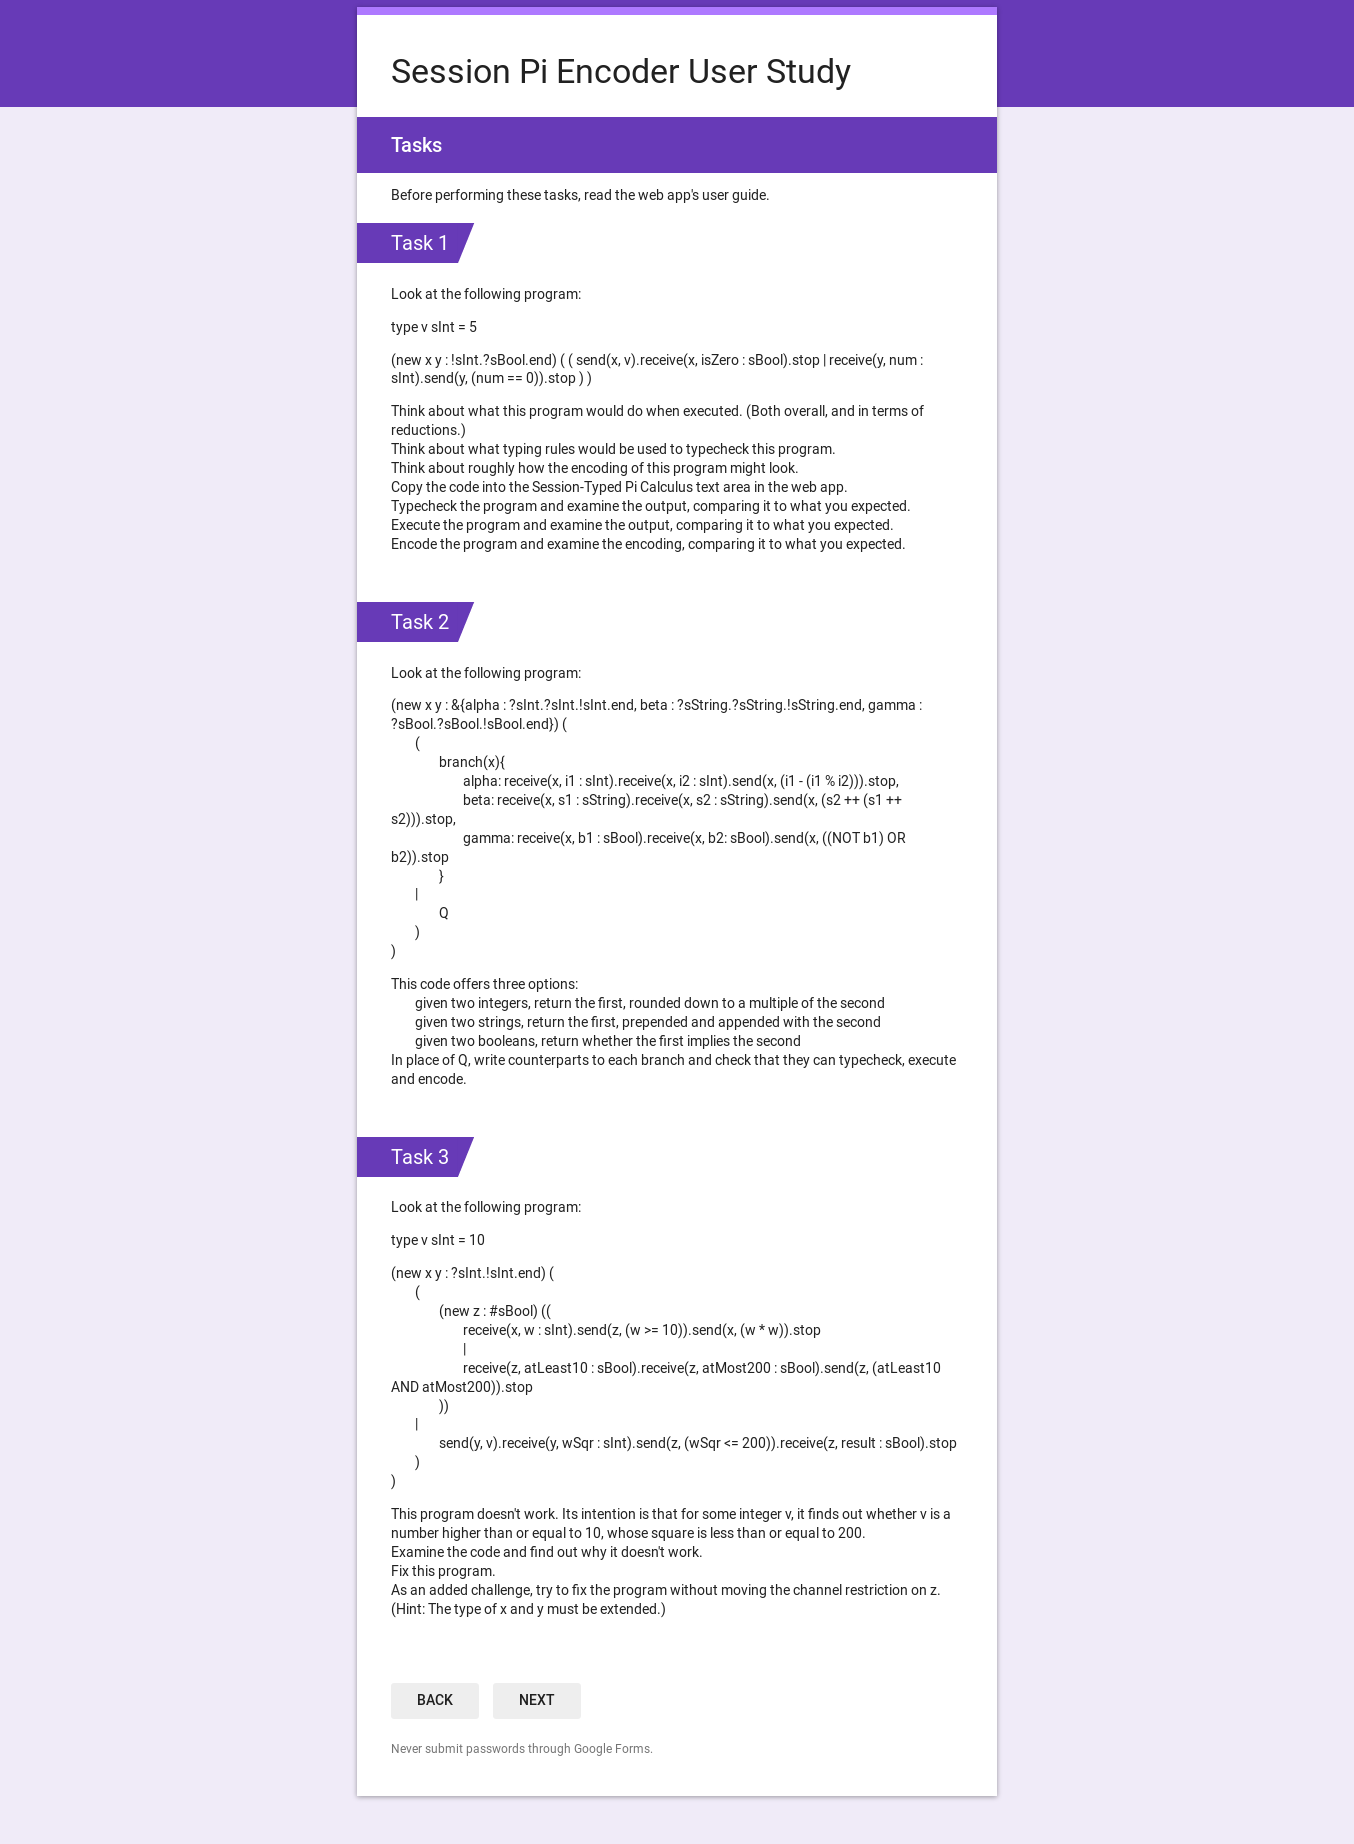
\includegraphics[width=0.72\textwidth]{images/SurveyPart2.png}
\caption{The second section of the survey, containing the tasks to be completed in the web app.}
\label{fig:surveyPart2}
\end{figure}

\begin{figure}[H]
\centering

\includegraphics[width=0.72\textwidth]{images/SurveyPart3.png}
\caption{The final section of the survey, containing the questions used to gather the views of the participants.}
\label{fig:surveyPart2}
\end{figure}

\section{User Study Ethics Checklist}
\label{appEthics}

\begin{figure}[H]
\begin{subfigure}{\textwidth}
\centering

\includegraphics[width=0.72\textwidth]{images/EthicsChecklistPage1.pdf}
\end{subfigure}
\end{figure}
\begin{figure}[H]
\ContinuedFloat
\begin{subfigure}{\textwidth}
\centering
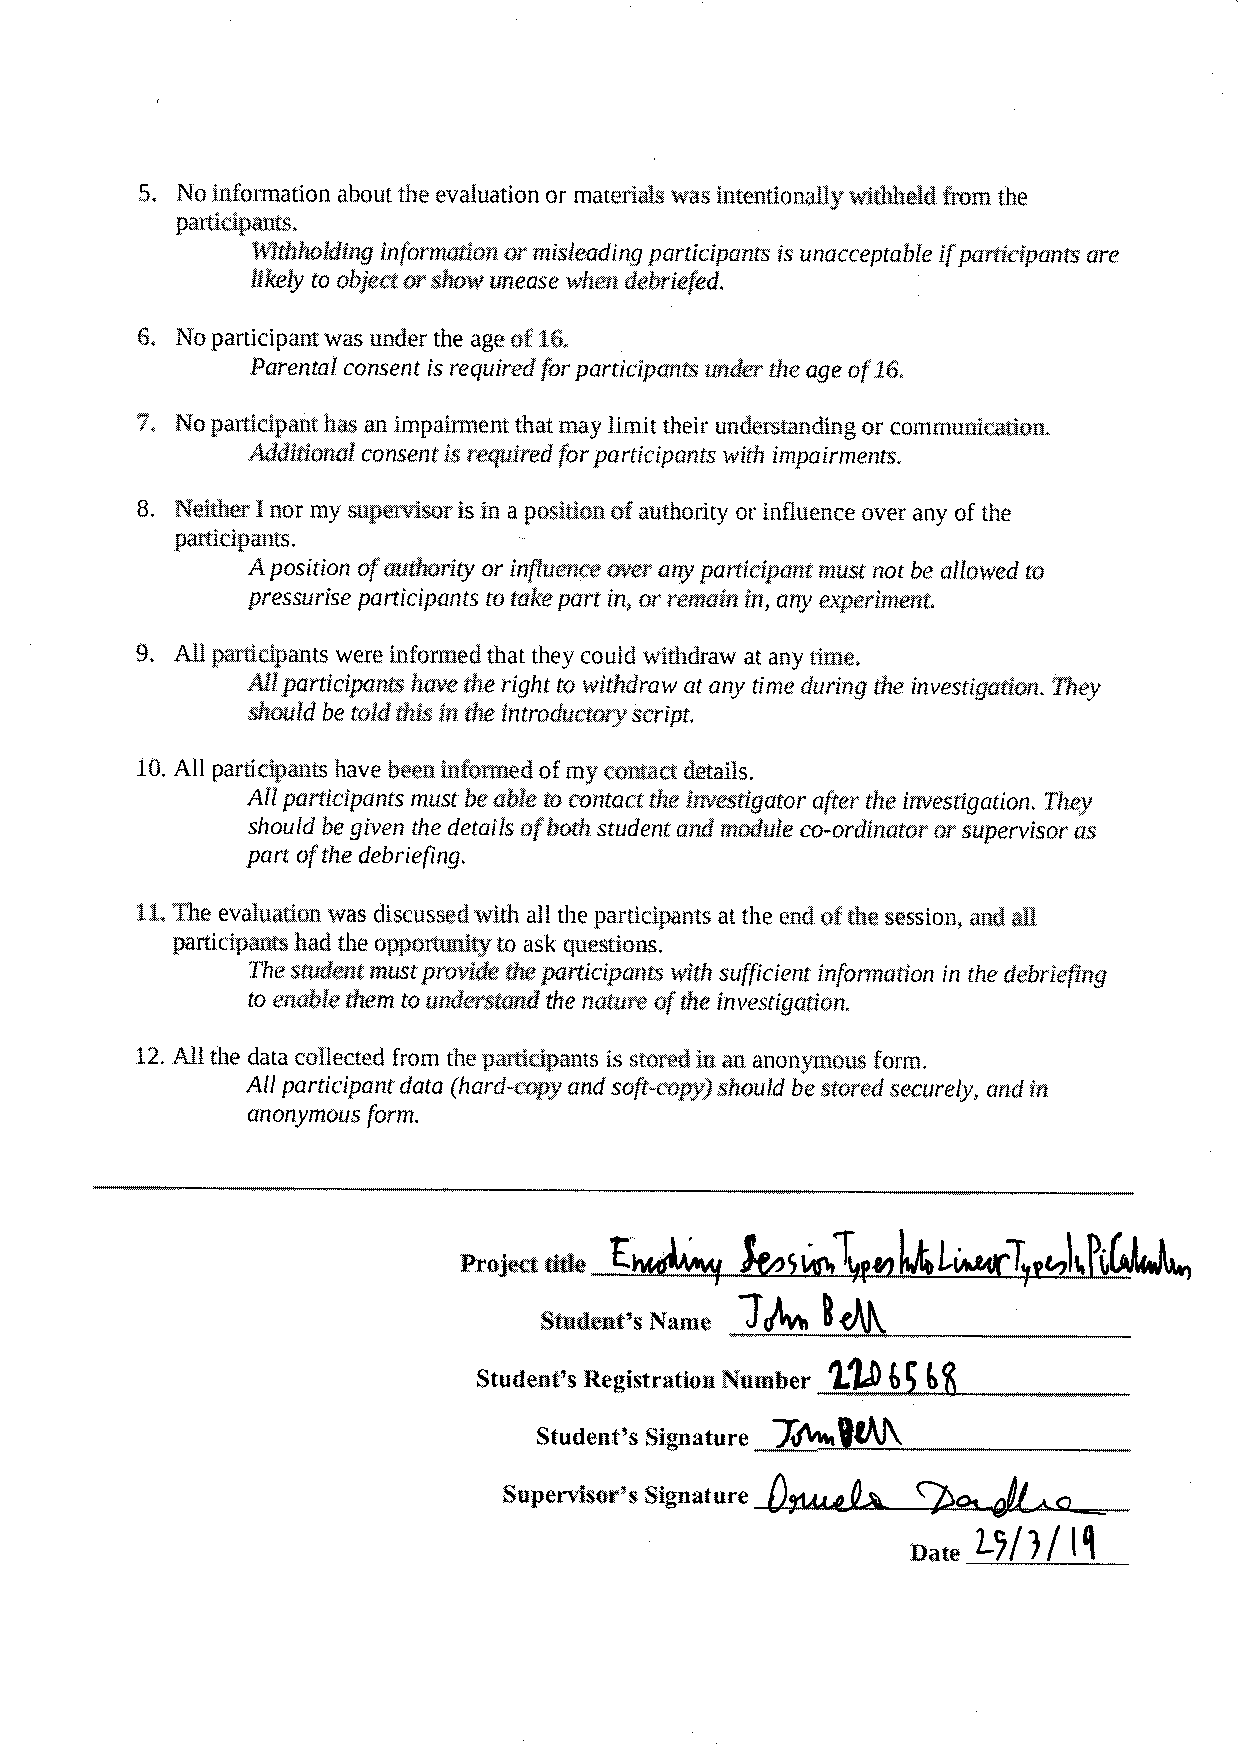
\includegraphics[width=0.72\textwidth]{images/EthicsChecklistPage2.pdf}
\end{subfigure}
\caption{The ethics checklist for the user study.}
\label{fig:ethicsChecklist}
\end{figure}

\section{User Study Introduction Script}
\label{appIntro}

\quad "The aim of this is to determine how usable and helpful this web app is for teaching people about $\pi$-Calculus and the encoding from session types to linear types. To do this, we need to show it to people and see how much it helped them understand those concepts. The survey starts with a few questions to work out how much you know already, then gives you a few tasks to complete on the web app and finally asks you some questions on how you felt about it. We're only recording your answers to the questions, not your performance in the tasks, so don't worry about how you do in those. Feel free to ask questions or withdraw at any point, and let me know when you're done. Do you agree to take part? And do you have any questions before starting?"

\section{User Study Debriefing Script}
\label{appDebrief}

\quad "Like I said before starting, the aim of this survey was to determine how usable and helpful this web app is in teaching people about $\pi$-calculus and the encoding from session types to linear types. Do you have any questions about any aspects of the survey? My email, and my supervisor's email are both on the form, so if you think of any questions, you can reach us through those. Thank you for helping."

\end{appendices}

%==================================================================================================================================
%   BIBLIOGRAPHY   

% The bibliography style is abbrvnat
% The bibliography always appears last, after the appendices.

\bibliographystyle{abbrvnat}

\bibliography{l4proj}

\end{document}
